\documentclass[a4paper, twoside]{report}

%% Language and font encodings
\usepackage[english]{babel}
\usepackage[utf8x]{inputenc}
\usepackage[T1]{fontenc}
\usepackage{tabularx}
%% Sets page size and margins
\usepackage[a4paper,top=3cm,bottom=2cm,left=3cm,right=3cm,marginparwidth=1.75cm]{geometry}
\usepackage{tikz}
\usetikzlibrary{shapes.geometric, arrows, positioning}
\usepackage{subcaption}

% Datetime
\usepackage[en-GB]{datetime2}
\DTMlangsetup[en-GB]{ord=raise,showyear=false}

%% Useful packages
\usepackage{amsmath, amsfonts}
\usepackage{graphicx}
\usepackage{MnSymbol}
\usepackage[colorinlistoftodos]{todonotes}
% \setuptodonotes{color=green}
\usepackage[colorlinks=true, allcolors=blue]{hyperref}
\usepackage{minted}
\usepackage{float}

\title{Robot Policy Learning with Active Vision}
\author{Kağan Uğur Pekgöz}
% Update supervisor and other title stuff in title/title.tex

\begin{document}

\begin{titlepage}

\newcommand{\HRule}{\rule{\linewidth}{0.5mm}} % Defines a new command for the horizontal lines, change thickness here

%----------------------------------------------------------------------------------------
%	LOGO SECTION
%----------------------------------------------------------------------------------------


\includegraphics[width=8cm]{title/logo.eps}\\[1cm] % Include a department/university logo - this will require the graphicx package
 
%----------------------------------------------------------------------------------------

\center % Center everything on the page

%----------------------------------------------------------------------------------------
%	HEADING SECTIONS
%----------------------------------------------------------------------------------------

\textsc{\LARGE MEng Individual Project}\\[1.5cm] % Name of your university/college
\textsc{\Large Imperial College London}\\[0.5cm] % Major heading such as course name
\textsc{\large Department of Computing}\\[0.5cm] % Minor heading such as course title

%----------------------------------------------------------------------------------------
%	TITLE SECTION
%----------------------------------------------------------------------------------------
\makeatletter
\HRule \\[0.4cm]
{ \huge \bfseries \@title}\\[0.4cm] % Title of your document
\HRule \\[1.5cm]
 
%----------------------------------------------------------------------------------------
%	AUTHOR SECTION
%----------------------------------------------------------------------------------------

\begin{minipage}{0.4\textwidth}
\begin{flushleft} \large
\emph{Author:}\\
\@author
\end{flushleft}
\end{minipage}
~
\begin{minipage}{0.4\textwidth}
\begin{flushright} \large
\emph{Supervisor:} \\
Dr. Edward Johns \\[1.2em] % Supervisor's Name
\emph{Second Marker:} \\
Dr. Adam Smith % second marker's name
\end{flushright}
\end{minipage}\\[2cm]
\makeatother

% If you don't want a supervisor, uncomment the two lines below and remove the section above
%\Large \emph{Author:}\\
%John \textsc{Smith}\\[3cm] % Your name

%----------------------------------------------------------------------------------------
%	DATE SECTION
%----------------------------------------------------------------------------------------

{\large \today}\\[2cm] % Date, change the \today to a set date if you want to be precise

\vfill % Fill the rest of the page with whitespace

\end{titlepage}

\begin{abstract}
Your abstract goes here
\end{abstract}

\renewcommand{\abstractname}{Acknowledgements}
\begin{abstract}
% Thanks mum!
\end{abstract}

\tableofcontents
\listoffigures
\listoftables

\chapter{Introduction}
Hello \cite{greenwade93}
\section{Objectives}
\section{Challenges}
\section{Contributions}
\chapter{Background}

% \chapter{Project Plan}
  In this chapter, I will cover:
  \begin{enumerate}
    \item What the project entails and how the work will be divided until the end of the project's timeline.
    \item The ultimate evaluation plan for the entire project once models are created and data is collected.
  \end{enumerate}

% Evaluation Plan
\section{Initial Plan}
I am keeping up with project tasks and deadlines in \href{https://linear.app}{linear.app} both for future reference and timestamping the work. Figure \ref{fig:linear} shows how that currently looks and more items will be added as they appear.

\begin{figure}[h]
  \centering
  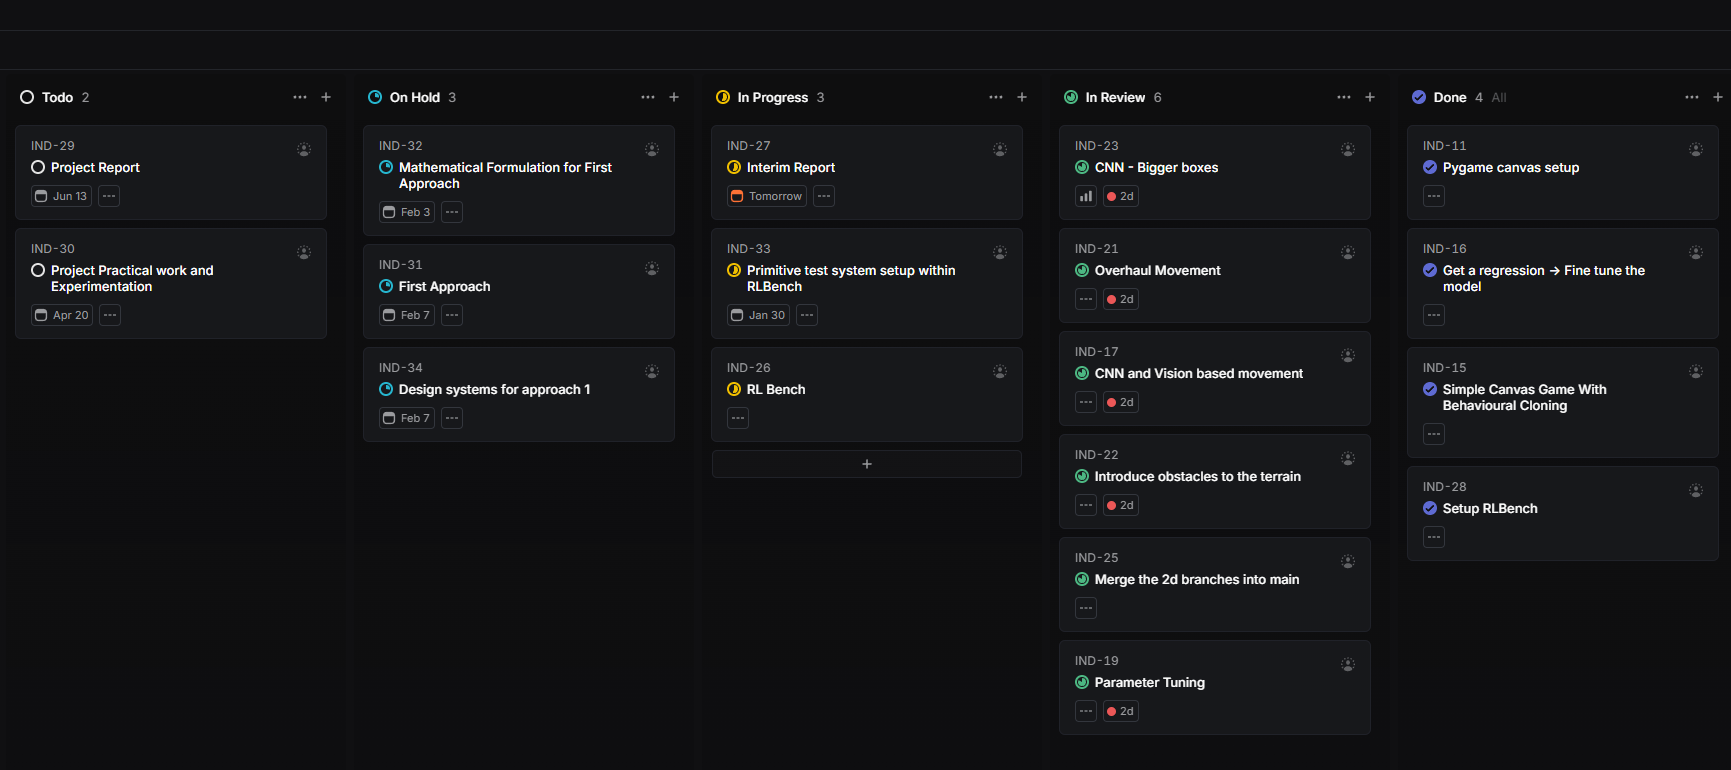
\includegraphics[width=\textwidth]{assets/initial-plan/initial-linear.png}
  \caption{Screenshot of the linear.app interface containing the first week deadlines}\label{fig:linear}
\end{figure}



\subsection{Road Map}
I am planning on dividing the project into little segments throughout the the term and the easter holiday. These will be in two week increments fo follow the frequency I meet with my supervisor. There are also some major tasks that are specifically deadlined. Such as, the hard report deadline \DTMdate{2025-06-13} (Top blue box in Figure \ref{fig:ggant}) and the internal deadline I set myself for the project experimentation is \DTMdate{2025-04-20} (second-from-the-top green box from Figure \ref{fig:ggant}). 
The experimentation deadline is designed to have a 10 day biffer and be able to accommodate overflowing to at max \DTMdate{2025-05-01}, so, the final month can be dedicated to making sure the report is comprehensive and complete. I aim to do report work throughout, and expect big updates on the report after experiment results and formulations.

Starting from the deadline of the interim: \DTMdate{2025-01-23}. Here is the outline of the first segment shown in Figure \ref{fig:ggant}.

\begin{figure}[h]
  \centering
  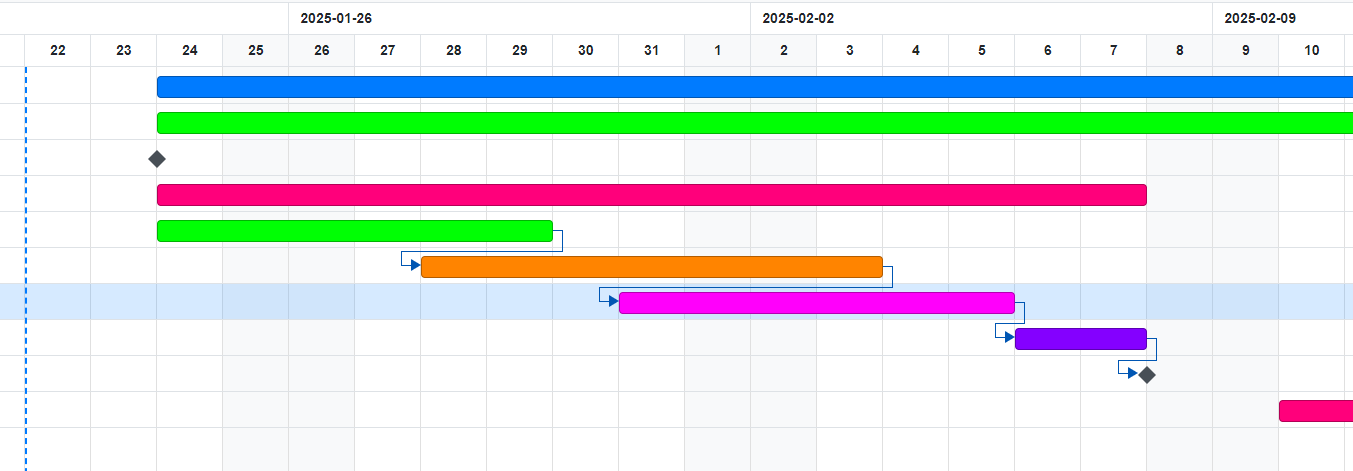
\includegraphics[width=\textwidth]{assets/initial-plan/first-week.png}
  \caption{Ggant Diagram outlining the first week}\label{fig:ggant}
\end{figure}

\subsubsection{First Milestone}
Initial plan is to create a rudimentary testing setup within \emph{RLBench} which is the benchmarking framework I started experimenting with (see more \ref{sec:eval-plan}). This is highlighted as the first green box after the first diamond shape in Figure \ref{fig:ggant}

Then, as discussed in the objectives (see \ref{sec:intro-objectives}), I am planning on starting mathematical formulation of the proposed approaches. Formulation will be the orange box. On completing formulation, I will move onto getting a system that attempts ideas from the formulation and possibly use the rudimentary testing system and test this in RLBench or other software as applicable. 

Then, finally, the dark purple box which is for writing out results before presenting to my supervisor on the next day.

\subsubsection{Later Sprints}
I don't expect every sprint to fit perfectly into the 2 weeks allocated. So depending on the size of the task and time it will require, I might allocate two sprints per task, totalling four weeks in total; or maybe half a sprint. Currently, I think this initial task, shouldn't take longer than about 12 days, hence I think a two week period is sufficient.

A quick high-level overview of the deadlines of other tasks are:
\begin{itemize}
  \item Have all approaches (again from \ref{sec:intro-objectives}) formulated and tried out on simulators to some degree by \textbf{\DTMdate{2025-03-15}}
  \item Have a finalised test environment that is robust and can hit criteria conclusively defined later(see \ref{sec:eval-plan}) by \textbf{\DTMdate{2025-04-20} [\DTMdate{2025-05-01} at the latest] }
  \item Have all testing done and report in a ready-to-submit shape by \textbf{\DTMdate{2025-06-01}} (leaving a healthy \~10 day buffer before submission)
\end{itemize}

Other local deadlines will be figured out along the way and will be tracked through linear.app, as mentioned, with minimum buffers of around a week for each, incase the work takes considerably more time than expected.
% Project Road Map
\section{Evaluation Plan}
\label{sec:eval-plan}
% \todo{note for evaluation, section on real-life testing and simulation tsting separately, to observe potential differences}
% As the project is an evaluation of the proposed framework upon adding active vision elements. It will have to be done on a pre-set collection of robot tasks. 
% Firstly, these tasks will be attempted with conventional approaches as control, either pre-trained open-sourced policies in a static-camera setting, or in-house policies without active perception. This will show us whether the improvements we suggest, in the form of extra learning and acting through active vision, has an affect on the success rate of the agents learning to do these tasks.

% On top of in-simulation testing, the 

I am currently planning to evaluate the policies I train on RLBench \cite{james2019rlbenchrobotlearningbenchmark}. A public benchmark designed for reinforcement learning algorithms and uses CoppeliaSim \cite{CoppeliaRobotics} in the backend.

CoppeliaSim is a mostly open-sourced, allowing the aforementioned RLBench, which is essentially a python wrapper to provide easy and programmatic access to the simulation environment. Also, in the long-run its realistic physics and rendering might allow our models trained there to be deployed in real-world environments, though will require additional verifications and the tests will not initially designed to accommodate this.

\subsection{Policy Performance}
The main focus of this project is to propose methods of active learning that are at least as good as static camera models in all scenarios and at least somewhat better (within the testing criteria) given some uncertainty for us to conclude whether active vision is a topic worth exploring.

\subsubsection{Baseline Evaluation}
Therefore, we need to establish some baseline policy performance, to be able to compare the outcomes of tasks. Some information we can evaluate are:
\begin{itemize}
  \item \textbf{Success Rate:} Percentage of times where the given scenario was executed correctly. Judged either by eye manually, or by some mechanism in the setup.
  \item \textbf{Failure Rate:} Similarly, ratio of runs where the policy doesn't complete the task satisfactorily
  \item \textbf{Time to Completion:} Mean time a policy, along many runs, takes to complete a task. 
  \item \textbf{Efficiency:} This will have to be explored to find what ``efficient'' would mean in the context of a benchmark. However, it could mean things like, how many steps to complete a reach-the-target sort of task (action efficiency), or path efficiency based on distance traveled to target etc.
\end{itemize}
These metrics will allow us to compare the active vision system proposed to baselines with different mounted camera positions.

\subsubsection{Inter-Active Benchmarks}
As we are planning on proposing multiple active learning policies, we should also have a method to compare them between each other. This comparison can use metrics such as:
\begin{itemize}
  \item \textbf{Camera Movement:} How much the camera moves in finding better viewpoints, can be expressed in terms of the total magnitude of movement at the end of an episode or run.
  \item \textbf{Frequency of View Changes:} This could give an insight into the policies \emph{sureness} or decision capability, choices that change the viewpoint frequently may hint at robustness issues.
  \item \textbf{Uncertainty Reduction:} Similar to above, as these policies are actively trying to decrease uncertainty in the given scene, it might be a good performance comparison to see entropy changes per model.
  \item \textbf{Occlusion Avoidance:} As this is one of the main topics advocating for active vision, we must characterise the performance of a model to avoid getting itself behind obstacles that might occlude goals. This might be defined in relation to the last two points covered above, or defined per task depending on the level of occlusion we place in a scene.
  \item \textbf{Success Rate in Occluding Scenarios:} Another follow-up point, using purposefully engineered tests that include multiple levels of occlusion, what success ratios can different models achieve. 
  \item \textbf{Novel Adaptation:} Comparing performance characteristics of completion of a task in different settings (such as different backgrounds) could give good insight about training scene generalisation. Or starting the robot in poses not demonstrated to check viewpoint novelty could give us good insight about a policy.
  \item \textbf{Noise Performance:} Similar to above, we can also experiment with noise such as varying lighting levels of the scene or different textures on objects to see if these can cause more failures and whether active perception will tackle random noise addition.
  \item \textbf{Simulation to Real Life:} Finally, if the project gets to the level of using these models in real-life, we can tests for the sim-to-real robustness and transferability of a policy by making it to the same tests in the simulation and real life and comparing some of these defining characteristics.
\end{itemize}

\subsubsection{Resource Utilisation}
Another section of the testing might include the acting performance of an agent compared to its computational performance. We can compare: \textbf{inference times}, \textbf{latencies is switching policies} between vision and motor (physical action) and maybe even \textbf{computational load} or \textbf{resource usage} depending on the architecture and its complexity. This might give us insight into the \emph{costs} of a performant policy.

\subsection{Initial Evaluation Proposal}
Although, we cannot create the entire benchmarking suite at this time, the general guidelines above will help us create a set of tasks that accurately assess the performance characteristics of our models. However, the suggestions above are in no way final and more can be added or some removed depending on relevancy of application to the test or benchmark.

\subsubsection{Basic Proposed Tasks}
As we are mainly concerned about active vision our tasks should include:
\begin{enumerate}
  \item \textbf{Navigation:} A path finding or reaching task differing levels of difficulty, such as: no obstacles, some obstacles to overcrowded and complex environments.
  \item \textbf{Grasping:} A classical example of a task we can explore the performance of a grasping task with policies such as eye-in-hand and a grasping task where the camera is decoupled from the gripper, but still active.
  \item \textbf{Searching:} This could be an interesting task, to test the limits of understanding coupled with a robots active abilities, for example searching for a ``red ball'' in a drawer of balls
\end{enumerate}

\subsubsection{In Simulation}
These tasks might look like the following in Figure \ref{fig:threesims}. However, these are currently suggestions and the test suite will not be limited to, nor be limited by the inclusion of these specific scenarios. These are just staring ideas for demonstration.

\begin{figure}[h]
  \centering
  \begin{minipage}{0.32\textwidth}
    \centering
    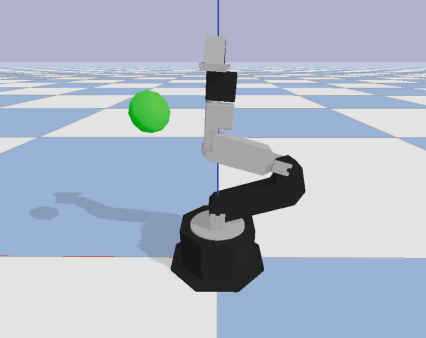
\includegraphics[width=\textwidth]{assets/eval-plan/reach-sim.png}
    \caption{Simple Simulated reaching task made in pybullet where the green orb is the target area, taken from \cite{aumjaud2020reinforcement}}
  \end{minipage}
  \hfill
  \begin{minipage}{0.32\textwidth}
      \centering
      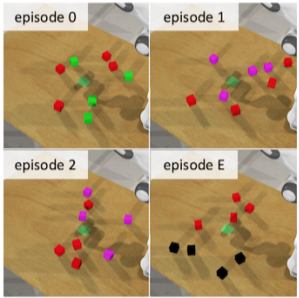
\includegraphics[width=\textwidth]{assets/eval-plan/grasp-sim.png}
      \caption{An example grasping task from RLBench \cite{james2019rlbenchrobotlearningbenchmark}}
  \end{minipage}
  \hfill
  \begin{minipage}{0.32\textwidth}
      \centering
      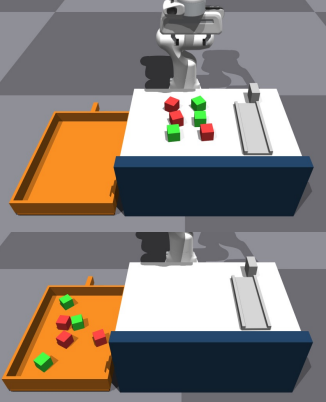
\includegraphics[width=\textwidth]{assets/eval-plan/search-sim.png}
      \caption{An example searching task from \cite{liang2022searchbasedtaskplanninglearned}}
  \end{minipage}
  \caption{Three Possible simulation tests, easiest level with no occlusions}\label{fig:threesims}
\end{figure}
 % //TODO: remove plan was for interim report

\chapter{Early Work}\label{ch:early-work}
In this section I will cover:
  \begin{itemize}
    \item Initial research and practical explorations in 2D 
    \item Laying the groundwork for 3D environments
    \item Problems when transitioning into 3D environments
    \item Early experimentation on limitations of robot vision
  \end{itemize}

% Early work 2d
\section{Early Work}
Early steps I was advised to work on was, getting an idea of \emph{learning} in two dimensions (2D) to get an intuition and follow it on with expanding it to three dimensions (3D) from there.

\subsection{Structuring the Problem}\label{subsec:ew-2d-problem}
Following those ideas I wanted to create a simple task to train a policy to teach a block to move towards the other block, on simple 2D rendered canvas. Essentially creating a two dimensional reaching task.

\subsubsection{Problem Design} 
I started with pygame \cite{pygame}, a python library that can be used to create 2D canvas with artifacts in it. But before rendering there are some things we have to define. I wanted to create a small\emph{ish} canvas to simulate the game in, with my player and target. I chose to make a $800 \times 600$ canvas and defined my blocks to be $20 \times 20$. Skipping the details the simple game was rendered as Figure \ref{fig:initial-canvas}, where the agent (blue) attempts to get to the target (red).

\begin{figure}[h]
  \centering
  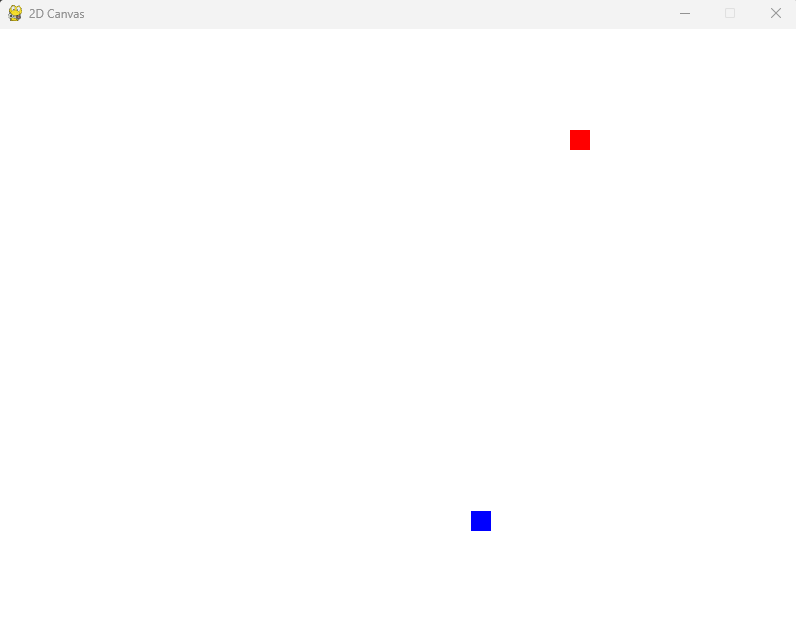
\includegraphics[width=0.6\textwidth]{assets/early-work/initial-canvas.png}
  \caption{Initial canvas $800 \times 600$ and $20 \times 20$ blocks}\label{fig:initial-canvas}
\end{figure}

As this was a simple game, for movement I defined a speed, which was initially $5$ pixels per press and mapped the movements to the arrow keys, and wrote a simple check that when the agent makes it to the target the game is complete.

\subsection{Solving the Problem: Learning}
To make a policy that would play the game, there was a few things I needed; firstly, the game needed a model to solve, I started with a classificiation approach, to classify the correct keys to press to move to the target.


\subsubsection{Classification}
Therefore, my model was fairly simple; the state, $S$ which is a \emph{4-tuple} $\langle float,~float,~float,~float \rangle$ that holds -in order- $x$-coordinate of agent, $y$-coordinate of agent, $x$-coordinate of target and the $y$-coordinate of target. And due to the keypress nature of the system, the Action, $\mathcal{A}$ was also a \emph{4-tuple} $\langle boolean,~boolean,~boolean,~boolean \rangle$ which was true or false to indicate if an arrow key was pressed, the positions in order are: \emph{Up, Down, Left} and \emph{Right}.

So, knowing the space, I created an expert policy, \(\pi_{demo}\), which gives the key combinations that must be pressed by interpolating where the target is with respect to the agent. Using their coordinates this was pretty simple. So, I randomly generated some starting positions and made the agent play the game many times and got snapshots of the states and stored them in a labelled structure for training a model later. \(data: list\left[State,~Action\right]\) where:
\[
  State:~tuple\left[float,~float,~float,~flaot\right], 
  \hspace{1cm} Action:~tuple\left[bool,~bool,~bool,~bool\right]
\]
as before. (Data loading was managed with dataframes and pickles for optimal GPU loading and speed)

Therefore, combining the two, I trained a linear neural network with 3 layers in PyTorch \cite{pytorch} predict the key presses (the action) given the coordinates of the blocks (state).

Without getting into implementation details, as this is early work, this worked pretty well. Every frame the state would be fed into the model and the model gives out the movement for that frame. Although, the movement was quite jagged because the classification was predicting key presses and the discrete actions were inherently not smooth; because a small change in a direction could prompt the model to change the  direction suddenly. A solution to this would be to get the direction change instead of a discrete movement direction. So, I pivoted to a regression model.

\subsubsection{Regression}
Similarly, as the scope changing I had to change my model slightly. State remained the same, but the action is now defined to have the type: \(Action: tuple[float, float]\), reflecting the change in $x$ and the change in $y$ (\(\delta x , \delta y\)).
Following a similar approach I now had a regression model, trained on the same data (also augmented to have coordinate labels)


\subsection{Extending the Problem: Vision}
To step the investigation in the direction of vision, now I wanted to do the same learning, however, without access to the coordinates of the blocks. I wanted to keep the regression interface, as the smooth movement was working a lot better and, in an ideal robot scenario in the real-world regression based actions are more common due to to continuous values in ranges of motion.

I started by creating my training data, this time as I was making the expert policy play the game, instead of saving the state as a \emph{4-tuple} of coordinates it was taking a screenshot of the canvas. As the canvas is an RGB image, the type of state now became: $State: list[Image, Action]$ where the image is a vector of size $3 \times 800 \times 600$, for the 3 RGB channels and the size of the canvas.

\subsubsection{Receptive Area}
Then I experimented with CNNs to be able to extract information from the scene and infer some sort of relationship. The first issue I faced was with receptive field size, I was mainly using a kernel size of 5 and stride of 2, so that by image was efficiently getting downscaled down the pipeline to learn information at smaller scales. 

However, due to the block size being too small compared to the total size of the canvas, CNNs that weren't deep enough were not performing well, due to not extracting features well. So I decided to increase the size of the blocks to $50 \times 50$ and after some experimentation and tuning parameters I landed on this model (Figure \ref{fig:cnn-5050}) that performed as well as, if not better, than the coordinate based regression model.


\begin{figure}[h]
  \centering
  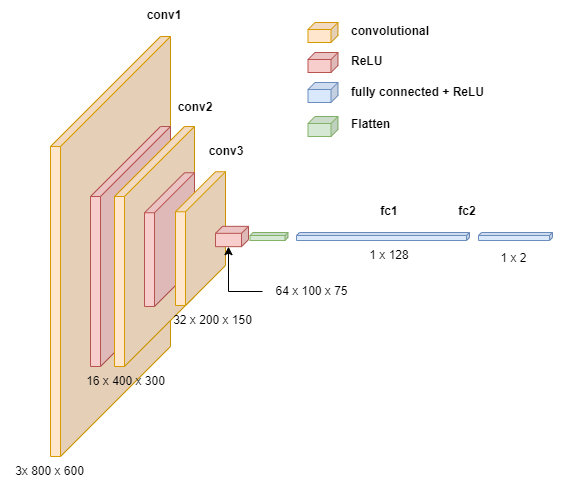
\includegraphics[width=0.8\textwidth]{assets/early-work/cnn-diagram.png}
  \caption{One of the best models for the agent reaching task}\label{fig:cnn-5050}
\end{figure}

\subsubsection{Sampling in Phases}
Another issue I ran into was the this model was performing generally well in getting very close to the target but refusing to take a very small step to collide and successfully complete the task. I realised this was because of the random sample collection being generally far away from the target, by the nature of uniform random sampling and there being vastly more space away from the target. So, to fix this, rather than changing the model architecture I changed the way expert data was sampled.

In training, I added a parameter to the training dataset, and to the creation of the training data. I made sure I could control the places data was being generated and labelling them where they were getting generated with respect to the the target. Called these phases of generation and made sure i could control the ratio of training samples and which phase they were coming from during the training. 

See Figure \ref{fig:phase-regions}, for an explanation of this idea. Giving more weighting to a closer region to the target, allowed my model to not suffer from the distribution shifts in my data, and allowed for the final push in the right direction for the agnet to complete the task successfully.

\begin{figure}[h]
  \centering
  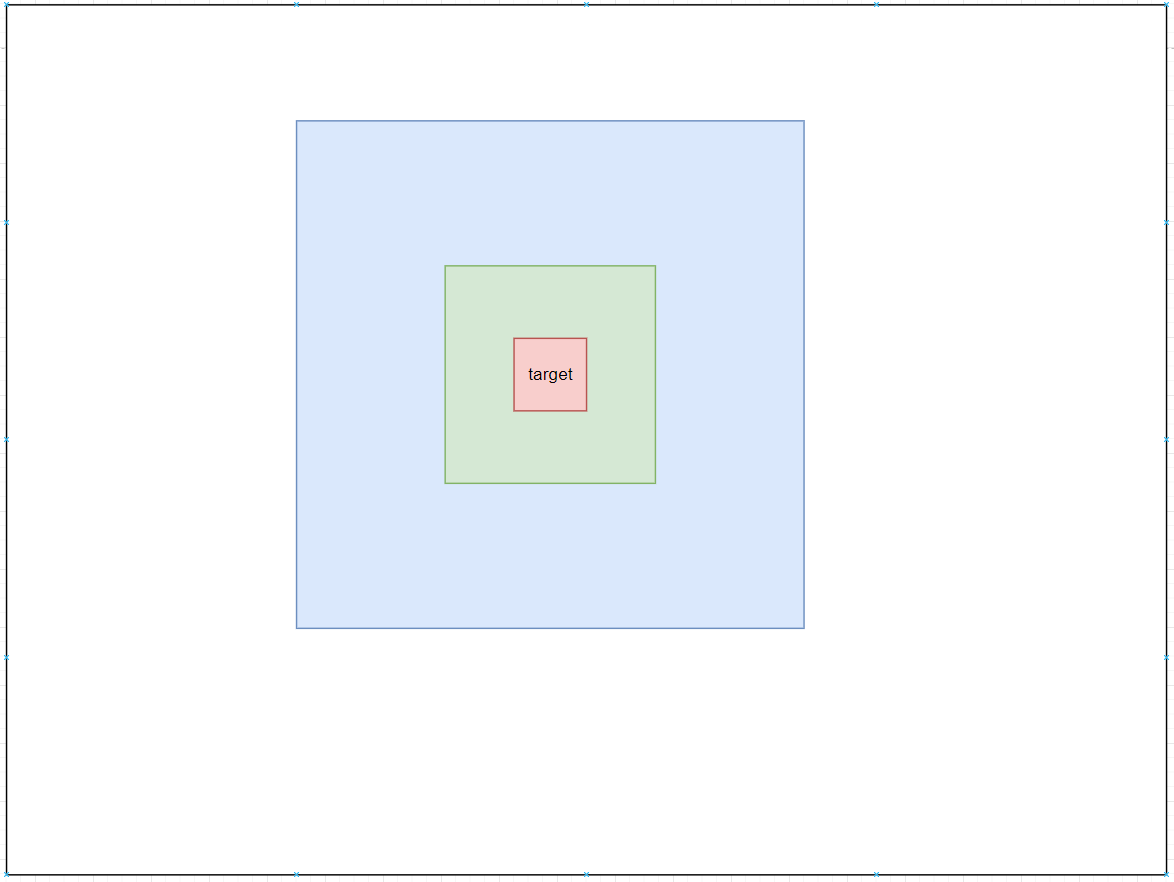
\includegraphics[width=0.8\textwidth]{assets/early-work/regions.png}
  \caption{Illustration of phases around the target, 0 would be green, 1 would be blue and 2 would be the rest of the canvas in this example. }\label{fig:phase-regions}
\end{figure}


\subsubsection{Returning to Small Blocks}
I also then got a model that was only one more convolutional layer deeper to work on the earlier smaller block size, however, the training time increase between the two were quite large for the same data sizes. Around one hour versus, four hours and change, for about 1000 episodes. Therefore, I continued this experimentation with the larger block size.


\subsection{Next Hurdle: Obstacles}
Then the next rational step was to add obstacles to simulate some ablations, which would mimic occlusions in 3D. Although, not visual barriers this was another hurdle the agent had to overcome.
Then the agent uses a path-finding algorithm, inspired by the $A^*$ algorithm \cite{cui2011based}, explores the cells around it with the heuristic of keeping the Euclidian distance of it and the target low.

\subsubsection{Obstacle Generation}
I took a simple procedural checkered approach where the canvas was divided into a grid which has cells the size of the agent. Then a cell will either be an obstacle or not with some clever mechanics around ensuring at least a single path from the agent to the target and some uncertainty. Check Figure \ref{fig:obs-gen} for some examples.

\begin{figure}[htbp]
  \centering
  \begin{subfigure}{0.45\textwidth}
      \centering
      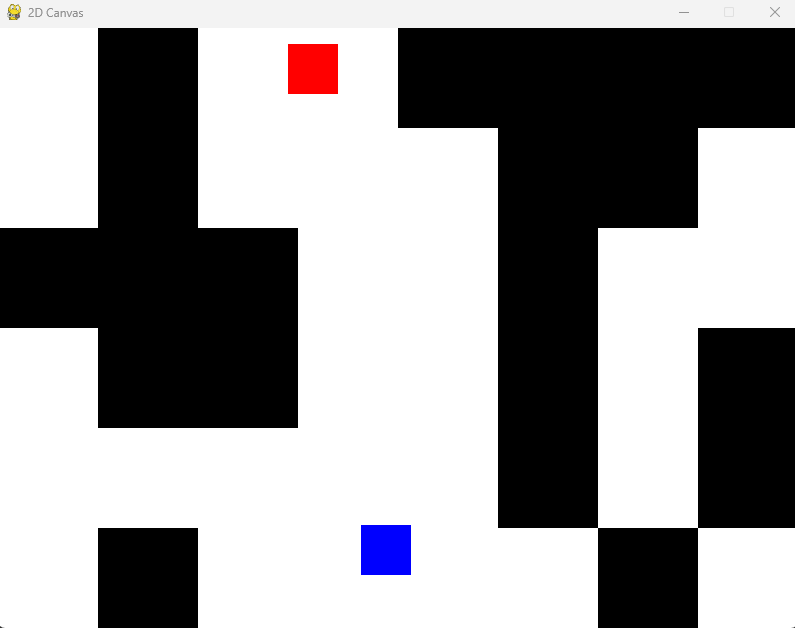
\includegraphics[width=0.8\linewidth]{assets/early-work/obs-gen1.png}
      \caption{Example 1}
  \end{subfigure}%
  \hfill
  \begin{subfigure}{0.45\textwidth}
      \centering
      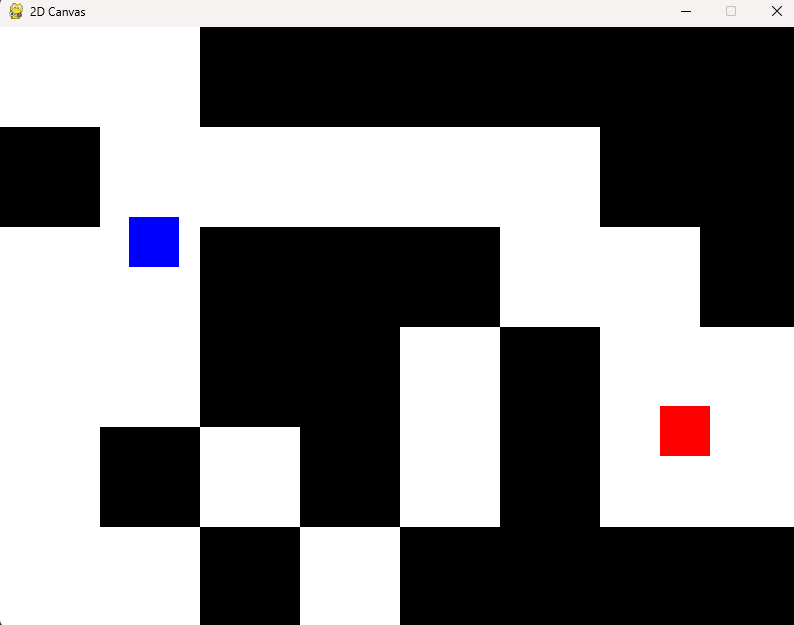
\includegraphics[width=0.8\linewidth]{assets/early-work/obs-gen2.png}
      \caption{Example 2}
  \end{subfigure}

  \vspace{0.5cm}

  \begin{subfigure}{0.45\textwidth}
      \centering
      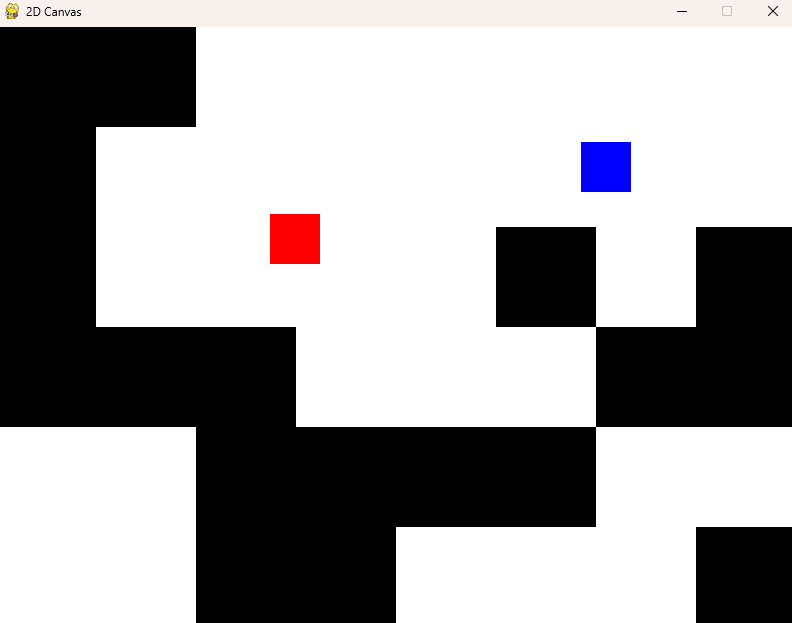
\includegraphics[width=0.8\linewidth]{assets/early-work/obs-gen3.png}
      \caption{Example 3}
  \end{subfigure}%
  \hfill
  \begin{subfigure}{0.45\textwidth}
      \centering
      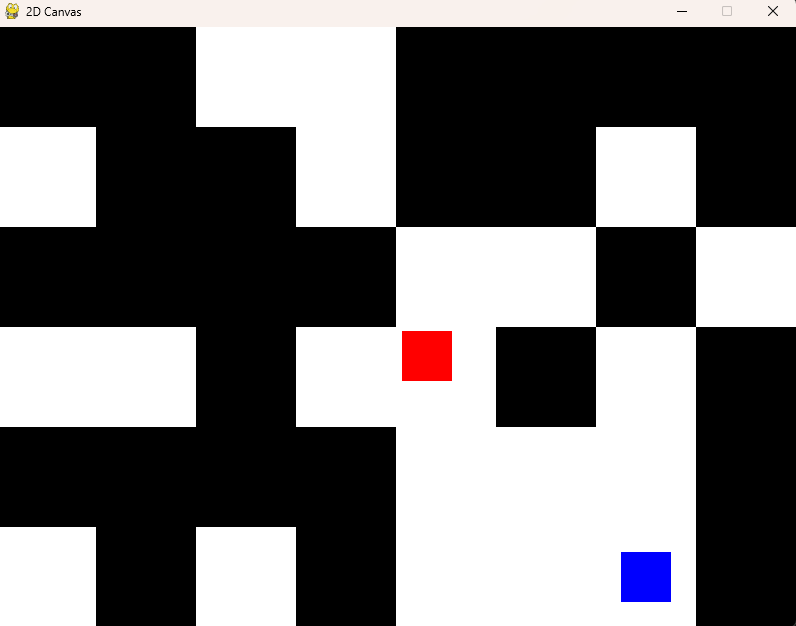
\includegraphics[width=0.8\linewidth]{assets/early-work/obs-gen4.png}
      \caption{Example 4}
  \end{subfigure}
  \caption{The 2 by 2 grid of some example obstacle generations}\label{fig:obs-gen}
\end{figure}\

\subsubsection{Getting Stuck}
I faced some issues with the model learning to avoid obstacles, the above policy for the no-obstacle case worked pretty well most of the time, however some select cases, such as there being an obstacle right between the agent and the target. 
\todo{figure for this, maybe for final report.} 

After some experimentation, I thought this might be because of the way I modelled the prediction system. Every frame expects a new movement to be generated, per the state given. This inherently has no history about where the agent was moving from. Similarly, the training data is also not ordered in any way, and it is frame corresponds to movement. Therefore, my model was essentially learning the underlying policy of the Euclidean distance heuristic used in the path finding and not extracting useful information about trajectories. This could have been solved with a reinforcement learning approach, or a demonstration requesting apoproach. Where the agent can ask for a new demonstration once it gets stuck or certain amount of time passes \todo{not sure here, talk about new demonstration and why I didn't do this?}

\subsubsection{Future of 2D: Sequence Models}
My next approach was to play around with a model that would take in multiple frames and output either one or multiple moves in order to have this idea of a history.

I experimented briefly with a \emph{sequence-to-movement} model primitively replicating a RNN, where it kept a 10 frame buffer along with the movement to predict the next movement. This idea seemed promising, however, my initial approaches were not fruitful, the models were suffering from a lot of empty episodes or repeated frames were causing erroneous learning. Therefore, I realised I had to pivot to non-concrete length sequences, such as transformer models accepting $n$ number of history frames with a max cap, rather than always needing the $x$ my makeshift-RNN was using (10 in my case). 

This is where I have currently left the 2D experimentation and moved onto starting some 3D approaches.


% Early work 3d
\section{Transitioning to Three Dimensions}
The move to 3D was slow, the jump from \emph{pygame} to a full blown physics simulation was a big leap and it came with its problems.

\subsection{CoppeliaSim and RLBench}

CoppeliaSim is a mostly open source simulation program that provides full access to its features through an educational license and RLBench \cite{james2019rlbenchrobotlearningbenchmark}is an in-house (Imperial) tool adapted to plug into CoppeliaSim through its python API interface, PyRep \cite{pyrep2020}. 

There are many tutorials online to help learn how CoppeliaSim operates and designing some scenes \todo[color=green]{maybe cite some stuff here, not necessary}. However, RLBench is a harder beast to tame. Although the system is very smart and it eliminates a lot of the required manual work before I can get started with running experiments; it is quite old, plugs into version $4.1$ of CoppeliaSim from 2020. As well as its age, I had had some issues setting it up on my system. 

\subsection{Environment Issues}\todo[color=red]{this section might need shortening, 2 pages is a lot for this}
One of the first large-scale issues I'd face in this project came here, quite early in its lifespan. I would soon learn robotics development is mostly done on Linux based machines and the journey to getting everything working would be quite long.

\subsubsection{Windows Setup}
I do most development work on Windows and WSL (Windows Subsystem for Linux) \cite{microsoftWSL} and expecting this project to be memory and graphic power hungry, it made sense to set everything up on the Windows side. This caused a few issues with PyRep, mainly because PyRep expected to be running on Linux, and RLBench was having issues launching.

\subsubsection{WSL Setup}
I thought this wouldn't be a problem, as WSL version 2 has been pretty good with GUI applications running on Linux and thought I could run Coppelia on there and still access any GUI (Graphical User Interface) I might need while developing tasks and observing my robot.

The translation layer between the operating systems might cause some slowing but there shouldn't be any major issues. Upon configuring everything as the installation guide suggested in RLBench and PyRep repositories. I had few issues linking object files downloaded with CoppeliaSim into the PyRep layer. After spending a lot of time researching issues, and coming across some online threads with similar issues (in different applications, so nothing was immediately applicable) I decided WSL must have been the problem and decided to move onto the next logical step.
 
\subsubsection{Linux Virtual Machine}
I had previously used Ubuntu a lot and even my WSL instance was running Ubuntu. As RLBench suggested Debian based systems, assuming they also developed it in Ubuntu, I created a Virtual Machine running it. After the entire setup process, I was finally able to get the instance running and finally managed to run one of the examples that gets downloaded when installing RLBench.

However, I got hit by another issues fairly quickly, the rendering of Virtual Box was definitely going through some sort of translation through Windows and the GPU adapted was not linking properly. So, everything was extremely sluggish, and running the non-primitive examples even crashed my virtual machine instances a few times. At this point I realised I had to settle for the real deal and got to partitioning by storage drive.

\subsubsection{Dual Booting}
I had some issues partitioning the drive Windows was already installed, so decided to get myself another drive I could boot Ubuntu from.

After running through the same setup steps and linking binaries, I was finally properly running RLBench. With one caveat, CoppeliaSim constantly complained that I was missing some video compression libraries; though seemed to work perfectly fine after installing them. It would always complain to me with a pop-up (see Figure \ref{fig:missing-libs}) but I found no issues with it during the project. There were other small annoyances like this throughout the entirety of the experimentation but finally I had everything working.

\begin{figure}[htpb] % htpb allows all placement
  \centering
  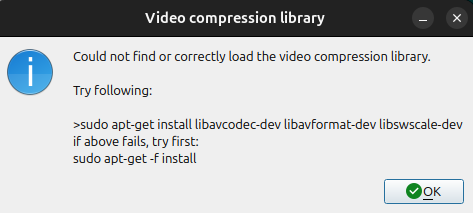
\includegraphics[scale=0.3]{assets/early-work/missing-libs.png}
  \caption{}\label{fig:missing-libs}
\end{figure}


\subsubsection{Campus Machines}
I knew that a solution to all of my problems might have been using a machine at the labs. I thought an issue with that may have been that RLBench needs some binary linking and setting of system variables, which might have required more access rights and the troubleshooting wouldn't be as easy as doing it on my machine. 

However, the main reason I didn't try this is because my personal machine has appropriately powerful hardware for a machine learning project and wanted to take advantage of this. So jumping through all these steps took about an entire week, but was well worth it, as now I have a system that can run all these systems in a headed manner, meaning I can watch and observe the behaviours of my robot as it learns and explores its workspace.

\subsection{Usability Issues}
One of the major instability issues I had was because RLBench is about 5 years old now and CoppeliaSim has moved on in some parts. However, PyRep didn not work with any other version other than version $4.1$ (2020), CoppeliaSim is now at $4.9$ (2025) \cite{coppeliaSimManual}.

\subsubsection{RLBench Codebase}
As I started using RLBench other issues started popping up, PyRep was randomly failing calls to CoppeliaSim due to errors raised in RLBench due to unexpected types and hitting exceptions such as \emph{``Should not be here''} which was especially frustrating. However, the solution was simple. Entirety of the RLBench source code is accessible, so instead of downloading it as a package I forked the repo and started fixing any issues as they started arising. Once trivial issues were getting fixed I also started using CoppeliaSim to make mockup tasks (see the next section, \ref{sec:3d-reaching-tasks}) and create networks that would use the simulation to train.

Around the time I started training some primitive models and learning more about these tools, I started hitting weirder errors, like the simulator constantly crashing, getting unexpected observation results, such as cameras such as overhead cameras  missing their input. Spending even more time combing though some of this \textbf{large} codebase I would sometimes find issues to fix them, but it would routinely break some of the package binaries I had linked and just stop working with no way to reason or figure out how to fix it. At this point I decided to check out some other tools.

\subsubsection{PyBullet}
The first option was PyBullet \cite{pybullet}, an open-source Python module for simulation, it wraps the Bullet SDK \cite{bullet3} and provides a completely customisable simulation experience. Though, the GUI experience is lacking and almost everything is controller through this SDK through a C-API
. 
Following some rough tutorials and combing through the manual for the module, I was able to put together fairly simple graphics, and shapes to start creating some tasks. Although, I came to a halting realisation soon after. Which was that without a complete robot learning suite at my disposal I would need to figure out a lot of the systems from scratch. Such as camera placements and movement systems, seamless task creation and linking, environment management, demonstrations and so on.


\subsection{Toolset Dilemma}
Therefore, I faced a lot of issues with RLBench, however, the time I spent on it was too long and learnt how to fix any issues when they came up. It also provided niceties like requesting demos and wiring environment and tasks fairly seamlessly. This means that I can spend my time engineering models and systems for active policy learning rather than creating a robot learning suite.

On the other hand, PyBullet was customisable and overall was more stable; CoppeliaSim (and especially v4.1 had few issues which I couldn't seem to fix) but RLBench has made a lot of ground work, to just get started with the project.

So the main dilemma was, should I be wasting time making a comprehensive suite to fit my needs early on in the project before  continuing with the premise of the task, or stick with RLBench and solve issues as they arise.

Fixing all the OS dependent issues and getting it running, I decided to stick with RLBench, hoping that the initial setup and early work issues would be the bulk of them. I also got familiar with the codebase during this time and was more confident in fixing any issues.

\section{First Steps in 3D: Reaching Task}\label{sec:3d-reaching-tasks}
Landing back on RLBench and solving most of the issues, first steps were to create some 3d environments and tasks to test capabilities of simple policies on tasks that progressively get more difficult. So, the very first step was to directly translate the 2D task I played with earlier in \ref{subsec:ew-2d-problem}. So, I created a simple reaching task. 

\subsection{Creating the Task}
As discussed before\todo[color=green]{where is this? link}, RLBench provides an intuitive method for quickly creating and validating tasks. Following the tutorials provided by the creator of RLBench and other resources online on CoppeliaSim \todo{link some copsim manuals or information here.} I could now create tasks for my use case.

Tasks are created using the \emph{`task builder'} CLI, which is a user facing interface that talks to the PyRep API which in turn controls CoppeliaSim. This allows the user to use GUI elements within the simulator to create objects, boundaries as well as edit their properties while observing what they look like in different camera view layers. Then to create scene wirings; the automatically created \verb|Task| class is used, where \emph{initialisation}, \emph{episode step} and other task related systems can be created for the scene object to then use to create demonstrations and train robot policies. See Figure \ref{fig:task-builder}.

\begin{figure}[htbp]
  \begin{subfigure}{0.48\linewidth}
    \centering
    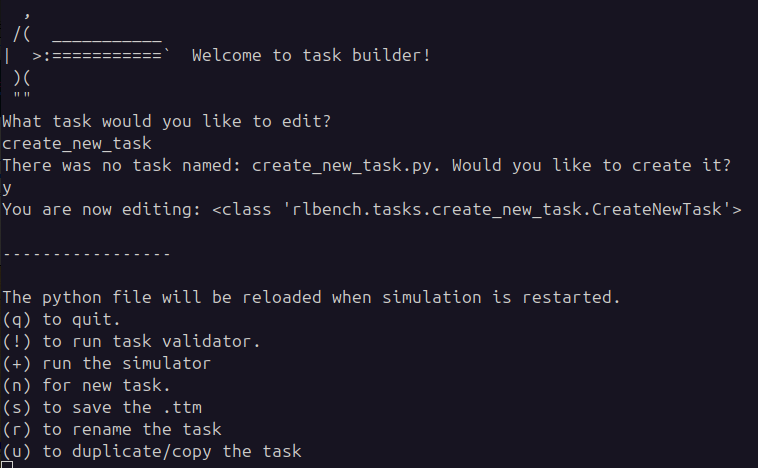
\includegraphics[width=\linewidth]{assets/early-work/task-builder-cli-1.png}      \caption{Task builder CLI: creating a new task}
  \end{subfigure}%
  \hfill
  \begin{subfigure}{0.48\textwidth}
    \centering
    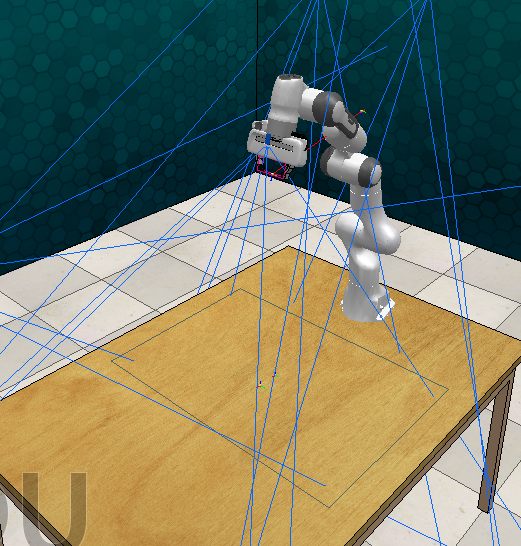
\includegraphics[width=\linewidth]{assets/early-work/task-builder-scene.png}
    \caption{Simulator: Graphical view of the new task}
  \end{subfigure}%
  
  \vspace{0.5cm}
  
  \begin{subfigure}{0.48\linewidth}
    \centering
    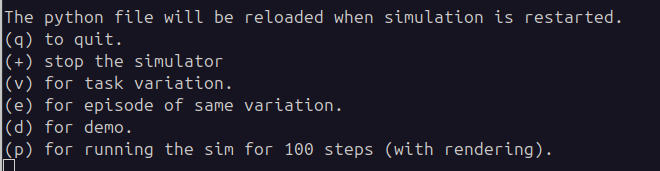
\includegraphics[width=\linewidth]{assets/early-work/task-builder-cli-2.png}
    \caption{Task builder CLI: running the simulator on new task}
  \end{subfigure}
  \hfill
  \begin{subfigure}{0.48\textwidth}
    \centering
    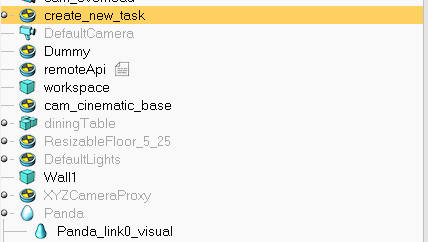
\includegraphics[width=\linewidth]{assets/early-work/task-builder-scene-hierarchy.png}
    \caption{Simulator: Scene Hierarchy of the objects in the new task}
  \end{subfigure}
  \caption{Creating a new task with `task builder'}\label{fig:task-builder}
\end{figure}\


The task I created is simple, see Figure \ref{fig:reach-no-obs}. I decided to use the \emph{Panda arm}, as that seemed to be standard and more importantly immediately supported by RLBench. It has 7 Degrees of Freedom (DoF) and a gripper -so the action space is a 8 dimensional vector. Then a red spherical target, which is not tangible, in the simulation it will be visually rendered but the arm will not collide or interact physically with it. Finally, added a proximity sensor to the target (which is not visually rendered) so the task can be immediately classified as completed by the system.



% //NOTE: relative paths for images, maybe add submodule once project is finished
\begin{figure}[htbp]
  \begin{subfigure}{0.48\linewidth}
    \centering
    \includegraphics[scale=0.4]{../fyp/assets/task-pics/reach-no-obs/random-front.png}      
    \caption{Front View}
  \end{subfigure}%
  \hfill
  \begin{subfigure}{0.48\linewidth}
    \centering
    \includegraphics[scale=0.4]{../fyp/assets/task-pics/reach-no-obs/random-top.png}
    \caption{Top View}
  \end{subfigure}
  \vspace{0.5em}
  \begin{subfigure}{1\linewidth}
    \centering
    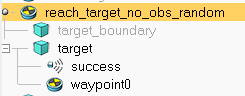
\includegraphics[scale=0.5]{assets/early-work/random-scene-hierarchy.png}
    \caption{Scene Hierarchy}\label{fig:reach-no-obs-hierarchy}
  \end{subfigure}%
  \caption{Reaching Task with no obstacles}\label{fig:reach-no-obs}
\end{figure}

\subsection{Creating a Policy}

The next step was to create a policy network. As I am mainly working on imitation learning from demonstrations provided by the system, my network needs to be able to ingest these demonstrations and generate actions in the action space of the robot. \par

\begin{center}
  \fbox{  
    \begin{minipage}{\linewidth}
      \textbf{Aside on RLBench Demonstrations} \par
      Demonstrations are provided encapsulated in a \emph{Demo} class and contain a series of observations (belonging to a class \emph{Observation}). These include state information of the robot and the environment, containing information like the observations of the set cameras and sensors; which need to be configured when the environment is started. This modular approach means I can collect demonstrations, then selectively choose what to use, like ignore a camera or a sensor. \par 
      Demonstrations are created following waypoints. PyRep expects  \emph{Dummy} objects within the scene called ``waypointX'' where sequence number of the waypoint starting from $0$. Then he demonstration engine calculates trajectories to these waypoints in sequence. For example, in Figure \ref{fig:reach-no-obs-hierarchy}, we have `waypoint0' within the target, for which a trajectory will be calculated from the tip of the robot gripper.
    \end{minipage}
  }
\end{center}\todo[color=green]{check centering acts weird sometimes}


\noindent By default the demonstrations -which I will refer to as ``demos'' from now on- and specifically the cameras pre-placed in the scene, produce images of resolution $128 \times 128$ pixels. I binned this down to $64 \times 64$. This comes in handy as I can keep the processing power low and can adapt the policy for higher resolution cameras by scaling it up later on. Therefore, I created a simple network following this architecture outlined in Figure \ref{fig:policy-arch}. The full code can be found in \todo{add the code of the network to appendix}.

\begin{figure}[h]
  \centering
  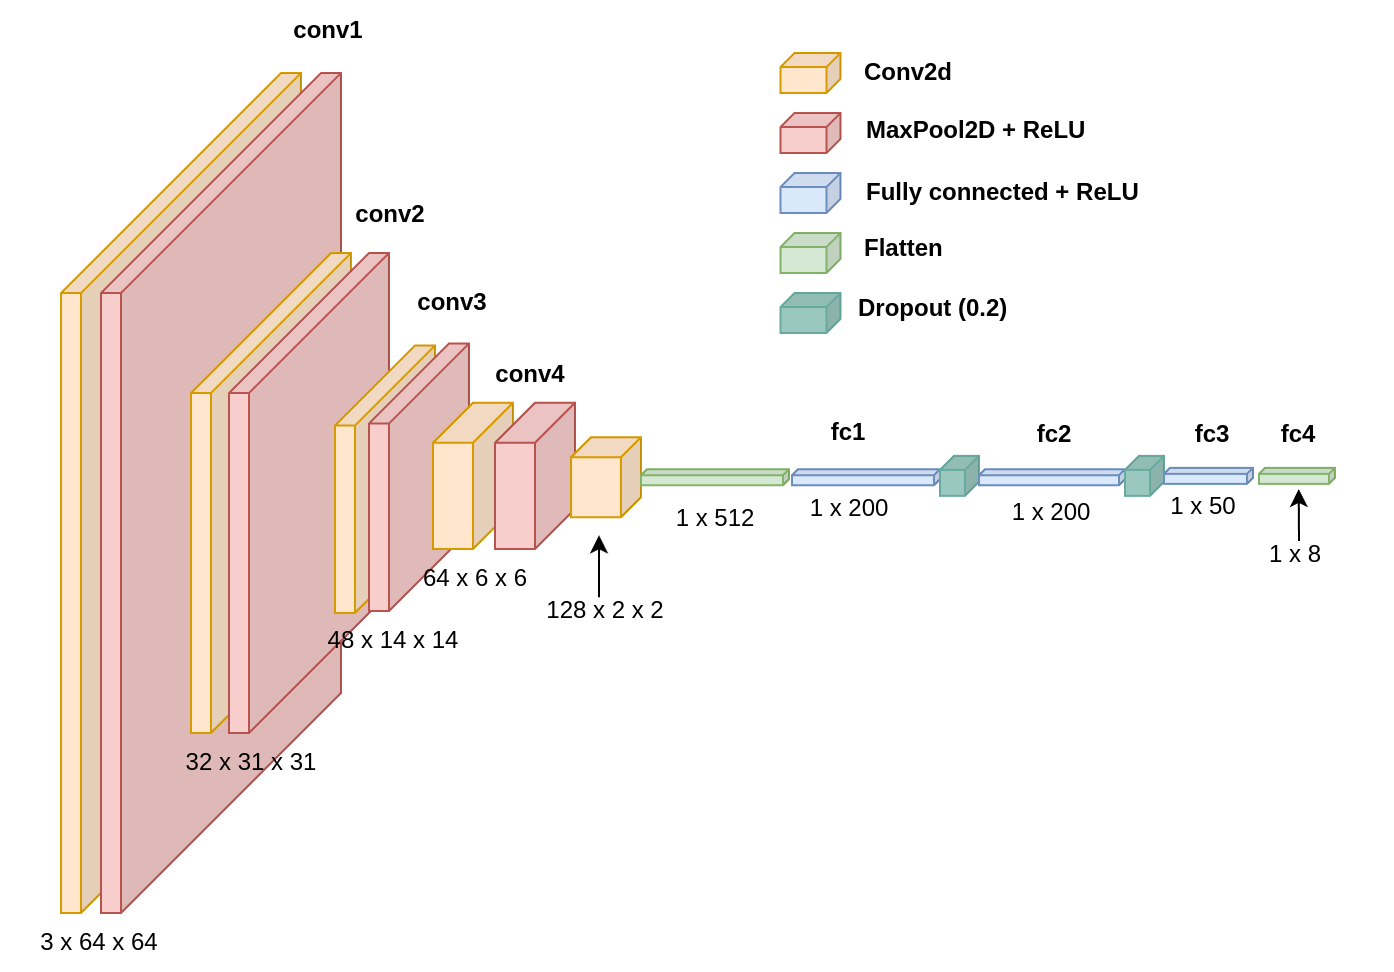
\includegraphics[width=0.8\textwidth]{assets/early-work/cnn-encoder-policy-head.png}
  \caption{Simple Policy Network Architecture}\label{fig:policy-arch}
\end{figure}\todo{ius the quality bad? reuload or reexport the xmml is in assets}


\subsubsection{Tuning the Policy}\todo{can remove not sure??s}
\todo{talk about the different types of ingesting state informariton per observation/per demo, run some tests , I think the per obs works better but find some reason as to why}

\subsubsection{Policy Improvements}
\todo{maybe do some lr scheduling and data processing for the images for generalisation  and mention the shuffling etc of the data and that it doesn't change much}



\subsubsection{Testing Visual Limits}\todo[color=red]{not sure about these to be honest, maybe remove these??}


conditions are not always ideal, so wanted to do some quick checks to get concrete results on how the agent behaves when the target is placed on the fringes of its field of vision. So created the three tasks shown in Figure \ref{fig:no-obs-3-views}.

\begin{figure}[htbp]
  \begin{subfigure}{0.3\linewidth}
    \centering
    
\includegraphics[scale=0.4]{../fyp/assets/demo-trials-no_obs/tasks/static-tasks-camera/initial-obs-side_l.png}      
    \caption{Left Side}
  \end{subfigure}
  \hfill
  \begin{subfigure}{0.3\textwidth}
    \centering
    
\includegraphics[scale=0.4]{../fyp/assets/demo-trials-no_obs/tasks/static-tasks-camera/initial-obs-central.png}
    \caption{Central}
  \end{subfigure}
  \hfill
  \begin{subfigure}{0.3\linewidth}
    \centering
    
\includegraphics[scale=0.4]{../fyp/assets/demo-trials-no_obs/tasks/static-tasks-camera/initial-obs-side_r.png}
    \caption{Right Side}
  \end{subfigure}%
  \caption{Three variations of the reach task with the obstacles sometimes out of view}\label{fig:no-obs-3-views}
\end{figure}

\subsection{Generalisability}
I had some static versions of this task where the target sphere was always in the same position, for which a single demonstration with long enough training is enough to learn the task. This is because without variation, Behavioural Cloning can be easily achieved by overfitting to the data. 

Therefore I created a dynamic version of the task, where the target is now randomly placed within view (not necessarily always fully within view but the centre will be, making sure the wrist camera can see it). This is achieved by using a \verb|SpawnBoundary| and randomly sampling the location of the target withing this for every new variation of the task, or for every new episode. Which can be seen in Figure \ref{fig:reach-no-obs}, the white bow being the boundary, which is not rendered in the simulation visually. This guarantees variety in demonstrations as well as helps us create a generalisable policy.

Running some tests with a tuned \todo{talk about tuning maybe?} policy, it was enough to see that, with the wrist camera having unobscured access to the target, it would easily learn to reach for it.


\subsection{Camera Limitations}\todo{reread and make sure it is a good starter segue to obs (maybe move these to after obs?)}

I was started experimenting limiting the learning to only the wrist mounted camera, which works well for this specific unobscured task, however, another interesting area of investigation is finding what kind of tasks benefit from different viewpoints, for example shoulder mounted or other static scene-observing cameras. 

Or more interestingly other sensors, such as depth or force sensors on robot hands or grippers. This relates back to the idea of human perception. To learn new tasks, we use all kinds of feedback from the environment that is reactive on our actions. Therefore, it is important to study shortcomings of individual sensors with respect to others to understand how policies with limited access to sensors can be made to overcome such challenges without necessarily adding more `observability' to a workspace.

\subsubsection{Multi Camera Mechanisms}
\todo{talk about `CamType' briefly}
\subsubsection{Policy Changes}
\todo{talk about the policy using differnt camera inputs to blend and make informed choices? maybe some plots here showing if it is better or not?}


\chapter{Feature Combination and Dependence Investigations}
This chapter I will be:
\begin{itemize}
  \item Creating some toy tasks in RLBench
  \item Propse methods of imitiation learning to solve these tasks
  \item Experiment with the strengths and weaknesses of said methods
  \item Augment my proposals with findings
  \item Use learnings to guide proposed active policies in the next chapter \todo{maybe remove this}
  
  \todo{there are commented notes from earlier here, might help the next section}
  % \item a good vision score policy without intrinsic information about the simulator.
  %   \item simple colour checking with a threshold?? -> shit but all that I could get working 
  %   \item  reay projectrion and checking if it lands on target
  %     \item  prior info about target?? -> using CAD models I can do RBG(-D) pose estimation
  %     \item extract prior information form demonstration?
  % \item segmentation masks to pull bits out
  %   \item  How do we know which segmentation mask is my target?
  \item 
\end{itemize}


\todo{in the vision experiments section add the condlusion from `plots.ipynb'  talk about why wrist is not generalising and the possible fixes by adding depth, }


\todo{move the depth interfacing here}
% Start
\section{Increasing the Toy Task Complexity}\todo{titles may need changing in this section}

\section{Reaching with an Obstacle}
So, to carry this investigation to the next level I introduced an obstacle placing mechanism as well as randomly placing the target behind the obstacle. This is to ensure that the agent doesn't learn where the target can be behind a wall from where the obstacle is. See Figure \ref{fig:reach-obs-random} for how this task looks and the check \todo{add appendix link} for the backend wiring of these tasks.

There are two versions of this task, I thought it might be interesting to randomise the object firstly dependently then independently on the obstacle. The `dependent' randomisation called \verb|ReachObs_Random| samples the obstacle, which in turn controls the spawn boundary of where the target can spawn in, meaning the target will always appear behind the obstacle albeit, edges of it can sometimes stick out. Conversely, the `independently' random version, called \verb|ReachObs_IndRandom|, this keeps the target spawn boundary fixed, meaning the target can be anywhere in the visible workspace, but it is not necessarily always covered by the obstacle. I can see that this potentially can be useful to keep the dataset a bit more diverse, and allow the wrist camera initially observe the target sometimes.

\begin{figure}[htpb] % htpb allows all placement
  \centering
  \begin{subfigure}{0.3\linewidth}
    \centering
    \includegraphics[scale=0.3]{../fyp/assets/task-pics/reach-obs/random-front.png}
    \caption{Front}
  \end{subfigure}
  \hfill
  \begin{subfigure}{0.3\linewidth}
    \centering
    \includegraphics[scale=0.3]{../fyp/assets/task-pics/reach-obs/random-side.png}
    \caption{Side (Left)}
  \end{subfigure}
  \hfill
  \begin{subfigure}{0.3\linewidth}
    \centering
    \includegraphics[scale=0.3]{../fyp/assets/task-pics/reach-obs/random-top.png}
    \caption{Top}
  \end{subfigure}
  \vfill
  \begin{subfigure}{0.45\linewidth}
    \centering
    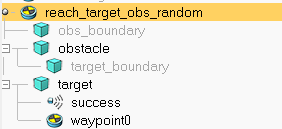
\includegraphics[scale=0.5]{assets/early-work/obs-random-scene-hierarchy.png}
    \caption{`ReachObs\_Random' Scene Hierarchy}
  \end{subfigure}
  \hfill
  \begin{subfigure}{0.45\linewidth}
    \centering
    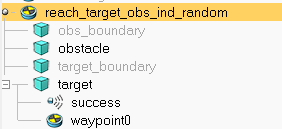
\includegraphics[scale=0.5]{assets/early-work/obs-ind-random-scene-hierarchy.png}
    \caption{`ReachObs\_IndRandom' Scene Hierarchy}
  \end{subfigure}
  \caption{Reaching Task with an Obstacle}\label{fig:reach-obs-random}
\end{figure}


\subsubsection{Wrist Camera Alone isn't Enough}

As expected, this is where the single wrist camera started showing its shortcomings. 

\todo{add graph of going around the obstacle but not quite reaching the target (wrist)}
\todo{show this with other combinations of cameras, comment on if the l/r without wrist can learn to go around the obstacle easily? maybe not, generalisation might be hard with no wrist}

The agent would easily move around the obstacle, however, would struggle to make the last steps in touching the target. This is mostly due to the fact that the demonstrations (which are provided by RLBench) are not necessarily pointing the wrist of the robot and hence the camera mounted there to look towards the target. This means that the wrist camera alone does not necessarily move towards the target, rather the robot learns to move behind the obstacle and nothing else.

From experiments I have realised that it learns to move around the obstacle easily, using simple behavioural cloning. However, getting the last nudge to actually reach the target is where it falls apart, especially in more realistic scenarios where the target is randomised behind the obstacle.

\subsubsection{Other Cameras}
Introducing the other cameras placed around in the environment, such as the \verb|left shoulder| or the \verb|right shoulder| cameras we can confirm that the wrist camera alone is not sufficient \todo{insert figure here with wrist vs others }, and the combination of wrist and other cameras are almost always the best as more coverage of the workspace guarantees less occlusions and more information the agent can work with to make decisions. It was clear that the wrist camera alone wasn't going to cut it unless it learnt to look towards the target.

\subsubsection{Implementing `Looking' into the Demonstrations}\todo{haven't done this yet}\label{ew-looking-at-target}
issues this is not easy might be working on this as a part of approach 2 later
Another solution might be to experiment with the demonstration system to make sure we are pointing the wrist camera (so, the hand of our robot) towards its target as a demonstration trajectory is calculated \todo{explain that this proved tricky and might not even be worth it}

If we can't implicitly encode the `looking' information through the demonstration that means we will have to inject this information into our agent some other way. Another way to make sure agent understands to look at the target is teaching it to actively seek out its target, either following previous works such as \todo{find some prior info tracking works add ref} where object priors are incorporated into the learning or with attention mechanisms that figure out what is important in a task without prior object information \todo{maybe reference this later}.  

\section{Expanding the Task Space: Grasping Tasks}
Another task which is likely to suffer from lack of viewpoints is a grasping task. So I designed these tasks around the idea of grasping. Firstly, a simple version (Figure \ref{fig:grasp-simple}) which the agent learns to reach then grasp the cubic target. 

Main differences between this and the reaching task is that the target here is tangible, so on top of being rendered it is also set to be \emph{collidable}. Another major addition is the usage of the \emph{extension string} as seen in \ref{subfig:simple-zoom-actions}, this instructs the demonstration engine to insert certain moves within the movement of the simple trajectory. In this case \verb|open_gipper()| ensures the gripper is open, then a later waypoint will instruct it to close.

\todo{maybe some experiment resutls here?}

The more complicated counterpart, shown in Figure \ref{fig:grasp-move}, is a scenario where the cube needs to be picked up then moved to the target location (designated in green)

\begin{figure}[htpb] % htpb allows all placement
  \centering
  \begin{subfigure}{0.3\linewidth}
    \centering
    \includegraphics[scale=0.2]{../fyp/assets/task-pics/grasp/simple-front.png}
    \caption{Front}\label{subfig:simple-front}
  \end{subfigure}
  \hfill
  \begin{subfigure}{0.5\linewidth}
    \centering
    \includegraphics[scale=0.3]{../fyp/assets/task-pics/grasp/simple-front-zoom-gripper_actions.png}
    \caption{Zoomed, with gripper action}\label{subfig:simple-zoom-actions}
  \end{subfigure}
  \caption{Simple Grasping Task}\label{fig:grasp-simple}
\end{figure}

\begin{figure}[htpb] % htpb allows all placement
  \centering
  \begin{subfigure}{0.45\linewidth}
    \centering
    \includegraphics[scale=0.2]{../fyp/assets/task-pics/grasp/move-front.png} 
    \caption{Front}\label{subfig:grasp-move-front}
  \end{subfigure}
  \hfill
  \begin{subfigure}{0.45\linewidth}
    \centering
    \includegraphics[scale=0.2]{../fyp/assets/task-pics/grasp/move-top.png}
    \caption{Top}\label{subfig:grasp-move-top}
  \end{subfigure}
  \caption{Grasping then moving}\label{fig:grasp-move}
\end{figure}


\missingfigure{grasp pic and possibly the demo gifs, }
\todo{add a picture with the cube grasped and the wrist camera view seen at that point}
Although, initially the wrist camera shouldn't pose any problems, as we advance through the task, especially after we have grasped something the wrist mounted camera becomes heavily obstructed and becomes unreliable so basing our decisions on this medium alone is not ideal.

\subsubsection{Observations}
What I got from these experiments was that the agent can benefit from understanding its surroundings at a higher level and more importantly remembering them. This is because once the camera becomes obstructed, as with \emph{Grasp Then Move}, even if the agent could do some exploration to find the target, it wouldn't be ideal due to the restricted view it has access to. So, observing the environment before, and remembering important parts will be vital for the later stages of tasks. I aim to explore some pre-policy visual exploration of the environment to be albeit to address issues such as this one.

\section{}
% Depth Interfacing
\section{Camera Dependence Investigations}\todo{does this warrant a whole new section or should I talk about it within obs and no-obs and grasp etc}
Following on from the earlier discoveries I wanted to dig deeper into the importance of different camera views and different sensors.

\subsection{Depth Interfacing} \todo{this is not done yet, gonna be a long week init}
\section{Depth Interfacing}
Another area of important research, before relating all this back to active vision, is figuring out distance. Depth interfacing is an important part of perception. Continuing from the drawn parallels to humans, we place object in our fields of vision by our two eyes. Stereo-vision, allows us to process two slightly different poses of a target object to reinforce our understanding of where that object is in the environment around us. Other information such as lighting (and shadows) may unconsciously help us as well. The main takeaway is that understanding distance to an object goes a long way in firstly understanding how to approach an object.

There are a few ways to achieve this in robotics. In RLBench specifically is either to use two cameras (with a known distance between the two cameras to adjust poses with known intrinsics). However, RGB cameras are not the only things we have access to. We also we have a depth sensor.

This is because, as I hinted earlier in the background section, the main idea of active vision is to be able to use minimal amounts of viewpoints and make the most out of these. In this scenario, I want to see if it can be justified to use the wrist camera accompanied by the wrist depth sensor to replace any other cameras we might have around the workspace. Paving the way to the next section in proposing active vision policies that act solely on information from a repositionable sensor.

Therefore, it is important to study shortcomings of individual sensors with respect to others to understand how policies with limited access to sensors can be made to overcome such challenges without necessarily adding more points of observability to a workspace.

\subsection{Grasping with Varying Depths}
To start investigating, I devised the following test task to see how the agent reacts to differently sized targets that might be placed at varying distances from the gripper within the scene

\subsubsection{Task Design}
A grasping task makes sense for this experiment. Because unlike the reaching tasks from earlier, the robot will need slightly more precision in executing its grasp and actually grabbing the target. The task performer needs to figure out where an object is before attempting to grab it. So, I created a modified version of the simple grasping task where the target object's distance and scale can be externally varied to observe the behaviours of agents in a controlled manner.\todo[color=green]{talk about delegating the task creating and param passing as well as the tasks in appendix and link here}

\begin{figure}[htpb] % htpb allows all placement
  \centering
  \begin{subfigure}{0.4\linewidth}
    \centering
    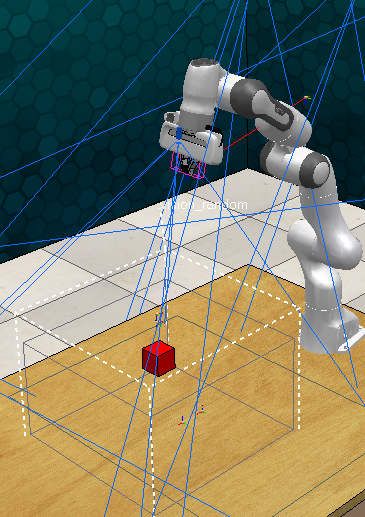
\includegraphics[width=0.7\linewidth]{assets/depth-interfacing/normal-size-grasp.png}
    \caption{Normal Target Size}\label{subfig:normal-grasp}
  \end{subfigure}
  \begin{subfigure}{0.4\linewidth}
    \centering
    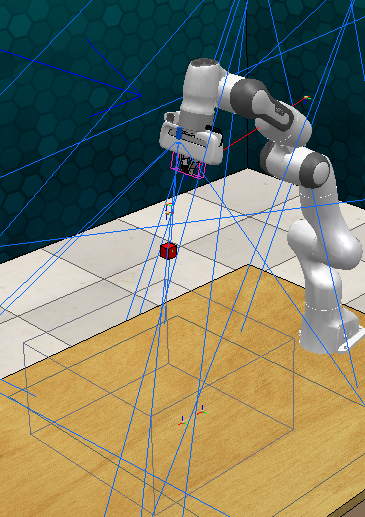
\includegraphics[width=0.7\linewidth]{assets/depth-interfacing/smaller-grasp.png}
    \caption{Smaller Target Size}\label{subfig:small-grasp}
  \end{subfigure}
  \caption{Visualisation of the Depth Interfacing experiment task}\label{fig:di-task}
\end{figure}

Figure \ref{fig:di-task}, is the general setup I am planning on using to evaluate the depth sensor versus a multi-view setup. Initial observations from the side clearly indicate that these are two different targets and will require different reach lengths before the agent can attempt to grab them.

\begin{figure}[htpb] % htpb allows all placement
  \centering
  \begin{subfigure}{0.4\linewidth}
    \centering
    
\includegraphics[width=0.7\linewidth]{assets/depth-interfacing/normal-size-wrist.png}
    \caption{Smaller - Wrist RGB}\label{subfig:normal-rgb}
  \end{subfigure}
  \begin{subfigure}{0.4\linewidth}
    \centering
    
\includegraphics[width=0.7\linewidth]{assets/depth-interfacing/smaller-wrist.png}
    \caption{Smaller - Wrist RGB}\label{subfig:small-rgb}
  \end{subfigure}
  \begin{subfigure}{0.40\linewidth}
    \centering
    
\includegraphics[width=0.7\linewidth]{assets/depth-interfacing/normal-depth.png}
    \caption{Wrist Depth Mask - Normal}\label{subfig:normal-depth}
  \end{subfigure}
  \begin{subfigure}{0.40\linewidth}
    \centering
    
\includegraphics[width=0.7\linewidth]{assets/depth-interfacing/smaller-depth.png}
    \caption{Wrist Depth Mask - Smaller}\label{subfig:small-depth}
  \end{subfigure}
  \caption{Wrist RGB and Depth Masks for the tasks}\label{fig:di-rgb-vs-depth}
\end{figure}

However, as seen in the comparison in \ref{subfig:normal-rgb} and \ref{subfig:small-rgb}, the RGB outputs look practically the same, and will very likely produce extremely similar features after extraction. A way to differentiate them would be to utilise the wrist depth mask in this encoding. As shown in \ref{subfig:normal-depth} and \ref{subfig:small-depth}, they now carry different features in those areas. In the depth mask the darker colours indicate closer objects, and the information is encoded as floats. 

\begin{figure}[htpb] % htpb allows all placement
  \centering
  \begin{subfigure}{0.40\linewidth}
    \centering
    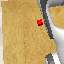
\includegraphics[width=0.7\linewidth]{assets/depth-interfacing/normal-l_rgb.png}
    \caption{Normal - Left Shoulder RGB}\label{subfig:normal-l-shoulder}
  \end{subfigure}
  \begin{subfigure}{0.40\linewidth}
    \centering
    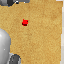
\includegraphics[width=0.7\linewidth]{assets/depth-interfacing/normal-r_rgb.png}
    \caption{Normal - Right Shoulder RGB}\label{subfig:normal-r-shoulder}
  \end{subfigure}
  \begin{subfigure}{0.40\linewidth}
    \centering
    
\includegraphics[width=0.7\linewidth]{assets/depth-interfacing/smaller-l_rgb.png}
    \caption{Smaller - Left Shoulder RGB}\label{subfig:smaller-l-shoulder}
  \end{subfigure}
  \begin{subfigure}{0.40\linewidth}
    \centering
    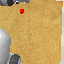
\includegraphics[width=0.7\linewidth]{assets/depth-interfacing/smaller-r_rgb.png}
    \caption{Smaller - Right Shoulder RGB}\label{subfig:smaller-r-shoulder}
  \end{subfigure}
  \caption{Left and Right Shoulder RGB Cameras}\label{fig:di-lr-shoulder}
\end{figure}


Another possible differentiating factor, and the reason earlier tasks were performing well, is due to the shoulder cameras. These also provide extra information about the scene the agent can use to understand its 3D geometry, even if it isn't explicitly taught. Although these are also not perfect, as seen in \ref{subfig:smaller-l-shoulder}, this camera is completely obstructed by the robot and is not seeing the target. This is not immediately problematic, because a smart enough system might be able to reason that the target is visible on the right and not on the left, leading to devising the correct depth for it. However, I have not intentionally encoded that information and doubt this network will be able to produce correct results with these observations.

\subsubsection{Adding Stereo Wrist Vision}\todo[color=blue]{can be removed not sure}
A possibility to overcome this \emph{self-occlusion} is to introduce stereo vision at the wrist level. Adding 2 off-centre cameras to the gripper, likely to the left and right of the existing wrist camera, will fix the self-occlusion, and possibly create a better comparison to the \emph{Wrist RGB} and \emph{Wrist Depth} combination. However, this comes with a lot of rewiring of RLBench and with its likely hidden issues that will pop up later. I did not want to take on this large architectural change before continuing with main investigation of the project, however, if timings permit this will be an important addition to the testing suite.



\chapter{Active Perception Policy Learning}\label{ch:appl}
In this section, by using what I have learnt so far, I will:
  \begin{itemize}
    \item Proposing some approaches to implementing active perception policies, mainly:
      \begin{enumerate}
        \item 3D Environmental reasoning policy
        \item View Uncertainty score policy
        % \item Human-like separate camera and gripper model for learning
      \end{enumerate}
    \item Discuss implementation details and ideas
  \end{itemize}

Contrary to the previous section, active vision entails moving the primary information source, as the robot control involves moving our robot (and by proxy its gripper) the cameras I will be mostly working with here will include some combination of the wrist mounted sensors, such as the RGB camera and the depth sensor.

% 1-
\section{First Approach: 3D Reasoning}
A problem we have with RLBench demos is that the gripper does not understand to look at the target. Therefore, in an occluded scenario the system needs to actively search for poses to make the target most visible.

So, rather than changing the training of the agent, I want to optimise its movement after training on demos.Which is to say, a policy will be learnt as normal using BC. Then during its execution, the robot can use 3D reasoning and  planning to move to its optimal state before applying what its learnt from the demonstration, increasing the chances of the BC algorithm succeeding in completing the task.

\subsection{Proposed Approach}
What makes this system is the \emph{optimal pose predictor}, as we want the robot to place itself in a situation where the:
\begin{itemize}
  \item Object visibility is maximised
  \item Occlusions are minimised
\end{itemize}
all the while keeping the robot in a valid kinematic state as dictated by the physics in the simulator.


A simple system would follow the following decision process:
\missingfigure{Train -> evaluate visibility -> if POOR: runu viewpoint optimisation, move gripper there -> execute trained IL policy}

We can formalise this optimal pose system as follows:
\[
p^* = {argmax}_{p \in \mathcal{P}}
  \left[
    V \left( p; \mathcal{O} \right)
    - 
    \lambda C\left( p \right)
  \right]
\]

Where \(p^* \in \mathcal{P}\), is a (reachable) candidate gripper pose, represented in in \(\mathbb{R}^7\): \( \left[ x, ~y, ~z, ~qx, ~qy, ~qz, ~qw\right]\), as RLBench stores pose information as a list of 3D coordinates (\(x, ~y, ~z\)) and a quaternion (\(q = \langle x, ~y, ~z, ~w \rangle \)) to represent rotation. Which is a more compact way of representing rotations compared to $3\times3$ matrices.

$\mathcal{O}$ is the given observation. So, any  3D information about the target object and the scene respectively. They can be mesh data about the objects, or possibly point clouds. This approach will initially have to depend on prior knowledge about the target, then later I might be able to encode the target information to be learnt during training so that we can remove the dependence on providing priors.

$V$ is the visibility score for our target object. We need to define some scoring functions to asses the utility of our current pose within the scene.

And finally, $C$, is some sort of constraint or cost function to help shape the choices correctly, it might be a constraint to make sure candidate poses are reachable, or maybe a cost function determining whether a candidate pose is too far from the current configuration. $\lambda$ is just a tunable weight to adjust how much these limitations contribute to out optimal pose finding. To add, there maybe multiple cost functions so we can expand them as: \(\lambda_1 C_1 + \cdots +\lambda_n C_n \).


\subsection{Implementation}
Following the plan, the most important part to start with is our utility function, and a way of sampling poses. Then I can start devising constraints to help shape the policy.

\subsubsection{Scoring a Candidate Pose}
The very first step is to implement an utility function. The initial plan was to use a pretrained segmentation network. Such as MaskRCNN \todo{ref?}. The idea was to segment objects present in the scene and ideally get some bounding boxes of where the system thought the objects were. 

Initial trials proved this problematic. Because, these networks were mainly trained with real-life data and pictures the toy tasks that I created without proper graphics overlaying them, would commonly be misclassified or not be classified at all. 

Along with bounding boxes MaskRCNN also gives uncertainties as well as the label of what it thinks this item is. Which I initially thought I could use as a score for `seeing' the target. From the wrist camera it would almost always find the grippers (which are visible) but it was quite uncertain at marking my main target object, and the very rare times it did mark it it would not be certain what it was. From the many pre-trained labels it would guess between: `apple', `fire hydrant', and `traffic light'. This is unideal because in the fully autonomous training stage, the network does not necessarily understand about what its looking for, and it doesn't care what its looking for. This however made it hard to quantify the \emph{vision score} with the uncertainty because firstly it couldn't decide on what it was, meaning I couldn't extract just a label from the MaskRCNN. Secondly,  it would sometimes latch onto other things in the scene, such as the grippers I mentioned (mostly identified them as \todo{i cant remember check again?}). So I either had to label these by hand, which is inefficient, or find a way to have the network learn what its target is through an unsupervised (or at least semi-supervised manner). 

Training my own version also seemed infeasible. Both because I would need a lot of annotated data on my specific tasks, which though doable would be time consuming. However, the main issue was the time. Spending time to tune and create the perfect feature extractor would waste precious time for the project. Considering the goals of this project, I moved away from this.

This therefore lead me to pursue a simpler definition of utility. As before \todo{ ref cam attn} I was going to extract the colour. However, had plans of integrating the point cloud data and incorporate depth into this score.

Unlike before, I didn't use a simple distance colour metric, but used a colour range. This achieves the same effect of extracting the target colours. However, I tuned the HSV high and low specifically to be more accurate. 

Another addition is the use of the wrist point cloud. We can create a spatial mask from the colour range to extract the depth information that is specific to the target region. We can extract points $k$ from \( {pc}^{world}\) where \(m_k \in \{ \text{True, False} \}\) as 

\subsubsection{Choosing a Candidate Pose}
Simple idea was exploration. The main reason my \emph{non-active} policies struggled was because the system would refuse to point the gripper towards the target. So I wanted to sample some poses and check if a pose around my current pose would generate a better pose, graded by the utility.

So, I wanted to limit my sampling on the surface a unit sphere of radius $\mathbf{r}$ where the current position of the gripper $\mathbf{c}$ lies ont he surface of. Therefore, the sphere's centre, $mathbf{O}$ can be found as \(\mathbf{r} = || \mathbf{c} - \mathbf{O} || \).

Once we have that centre, we can sample \(\phi \sim U\left(0, 2\pi\right)\) abd \(u\sim U\left(0, 1\right)\) then set \(\cos \theta = 2u - 1 = \arccos\left(2u - 1\right)\). Using these values we create the unit vector \(\mathbf{u} = \left[ \sin\theta\cos\phi, ~\sin\theta\sin\phi, \cos\theta\right]\) and \(\mathbf{p} = \mathbf{c} + \mathbf{ru}\). Next, we pick the `facing' direction of our orientation, it made sense to always point towards the centre of the sphere. Once all these are set, we need to find the orthonormal basis to fix the roll around the  `facing' axis we have chosen.\todo{ref code, this is boring geometry} Once the full position and hte orientation is established, we can return this 3D matrix back into the pose and quaternion representation, so, we have a sample to test. We can use the \emph{inverse kinematics} of our robot to find out what configuration the joint angles need to be. And with a simple velocity controller, I arbitrarily chose a simple proportional control module system\todo{ref appendix}. We can move our robot to that location.

An important note, I arbitrarily chose the sphere centre to be right below (with a distance $\mathbf{r}$) the gripper position. The inverse kinematics system would frequently not be able to get to the joint configurations for many different radius configurations provided, so, for the final version of this system I adapted the pose sampling to only sample orientations. Rather than changing the position, it would change the orientation of the gripper with a random rotation, and then as before solve it with inverse kinematics. This meant that no position exploration would be happening but the agent would more robustly explore different orientations. 

I initially utilised two constraints in the pose selection, kinematic distance to the next pose, calculated by the absolute joint rotation differences. \(C_{jpos\_dist} = ||\mathbf{p}_{sampled} - \mathbf{p}_{current}||\). And secondly inverse kinematics solver. If it cannot be solved, \(C_{ik}\) blows up and that pose will not be considered. The ik solving discouraged movement because the score is calculated after moving. However, the distance could not immediately be added, because we need to move before getting a observation and scoring it. Therefore, I decided to take only the top $k$ of the samples from the sphere, encouraging only closer movements. And for the only-rotation approach, I just removed the distance restriction. This is because a simple rotation will be cheaper compared to full movement.

In later iterations, with a view estimator and other predictive scoring mechanisms, we can introduce the distance again, as then the entire score calculation can be done without requiring movement.

\subsubsection{Collison Avoidance}
A final heuristic I added was using action smoothing and back-off if we were getting too close to an object. As we now have access to the projected point cloud from the wrist. And removing the the target from this point cloud.\todo{usign the above calculations} By sampling for the closest $k$ points in the point cloud I estimate the centre of the closest obstacle. And set a repulsion direction away from it.
Then with some extra parameters: \textbf{clearance} and \textbf{blend} is used to calculate the distance thresholds and how to smoothly transition from full repulsion to the full action. As the wrist camera can see the tips of the grippers, I made sure to ignore these, they are about $0.895$ metres from the camera, so I checked distances above this and below the clearance to act on this information. \todo{see how its done in appendix}


\subsubsection{Action Loop}
There are two actions loops. I equipped the \emph{active agent} with one of the good policies from the earlier chapter. Essentially, there would be an \emph{active action} and a \emph{BC action}. The toggle between the two settings will depend on the utility score and an arbitrary limit to how long the agent can explore will be placed, so that it doesn't get stuck somewhere forever.

I initially started in active mode, which means that agent would continuously search at the start. This is a bad system because the agent is no where close to the target nor the obstacle. And with only the rotational exploration, it wouldn't be able to move. So the next heuristic was that, the active portion would only kick in once we were close enough to the obstacle, and the vision score was low. The closeness was not euclidean distance but a z-height range, so that slamming into the obstacle form above does not trigger the active mode, which again would get stuck. The final decision system is given here \todo{figure:}
  
% 2- (barely exists)
\section{Second Approach: View Emsembling}
We still have the same problem of estimating the best pose for our gripper. Getting the agent to plan using its environment has the drawbacks of needing a lot of prior information about the task. Which leads to inherent coupling to tasks or environments.

What if we could inject the movement of the camera into the RLBench demo system, so the view uncertainty system can be modelled independently of the environment on the data we have received. In short the plan here is to get demos that have multiple observations per timestep (meaning multiple observation collections and not just multiple modalities.) Then we can train a model with inherent uncertainty models to estimate the best pose to be in before executing an action. In theory, this should help eliminate the need for geometrical priors.

\subsection{Proposed Approach}
The changed demonstration system will give demos as \( \mathcal{D} := \{\langle \{o_i^t\}_{i = 1}^{N}, a^t\rangle\}_{t = 1}^{T}\) for $N$ distinct observations per step in $T$, this will allow us to train an ensemble method with one or more of these observations (but not all) and leverage the information gained 

\subsubsection{Regression Ensembling}

\todo{math foundations, add other subheading for limitations such as adding movement within rlbench demos??}

\subsection{Implementation}
\todo{need to make something here not sure what yet but I need at least one thing to compare the main thing}
% 3 - (does not exist)
% \section{Third Approach: Separate Cam and Hand Control}
\todo{explain what this is}
Initial idea from my supervisor was to train a policy -using reinforcement learning- to train a policy that directly controls the camera, for any task and object. Then when the main policy is trained using imitation learning on the specific task from the human demonstrations, both policies can be deployed to make sure the robot is optimally observing areas of the task that might be of interest.

Even though this was the main objective of the project from the get-go, without the previous ground work and the clearer understadning of comparably simpler policies, this would have been very hard to start working on. This is why 

\subsection{Proposed Approach}
\todo{propose some plan, maybe talk about placing a second movable camera in the workspace}


\subsection{Implementation}
Due to its complexity, and frankly, running out of the limited time we are allowed for this project, I was not able to iterate on this approach to the same quality as the ones above, and produce a system that works using this plan.

Hence, this will not be in the final comparison, but being the main motivator of the project, this is what this project will naturally evolve into, if development were to be furthered in this area.

\todo{even if i get a shitty implementation of this, which is not happening i dont think, I will just say not good enough to add to results etc}
  

\chapter{Evaluation}\label{ch:eval}
Here I will evaluate:
\begin{enumerate}
  \item Findings from the FDC investigations
  \item Compare the proposed active vision approaches to non-active systems from before
\end{enumerate}\todo{split later if needed}

% Setuo
\section{Evaluation Setup}
The general setup included training a set of policies with their inherent hyperparameters, which will be discussed during their specific sections.

\subsection{Collected Data}
The data I chose to collect to reason about these policies are:
\begin{itemize}
  \item \textbf{Camera Type} A misnomer, indicates which sensors or combinations of sensors are being used in the policy to make decisions from \({RGB}_{wrist, ~left\_shoulder, ~right\_shoulder}\) and \(Depth_{wrist}\).
  \item \textbf{Final Distance} (to target) all of my tasks are target centric, so final distance within the allowed episode length a measure of competence.
  \item \textbf{Minimum Distance} (to target) as above. The difference is reasoning where a policy might be falling apart, seeing the discrepancies between \emph{min} and \emph{final}
  \item \textbf{Success Rate} All the tasks had slightly differing success criteria, however this is an important measure for competency again. This was mostly measured as a count out of $n$, for $n$ being the length of the test demonstrations. The term ``test demonstrations'' means that a set of demos were recorded with the target and the environment in a fixed state. Loading these back allows us to hae a comparable test between policies and their variables.
  \item Other policy specific hyperparameters that were relevant to observe. These will be discussed when relevant.
\end{itemize}

\subsection{Reproducibility and Verification}
All the random aspects that can be controlled, be it \emph{numpy} and \emph{pytorch} random choices or random `live' demos. Seeds are sets for both the libraries, as well as the \verb|DataLoader| seeds being fixed for the entirety of the policies tested here.
The demos per task are pre-made and saved in the project repository. \todo{ref the final deliverables bit}. I repeated all the tests with $5$ different seeds for the data shuffling, to observe if training on a different (but controlled) ordering of the demos affects a policy.

\section{Test Environments}
Two main branches of tasks I followed in this project are grasping and occluded reaching tasks.

\subsection{Reaching with an Obstacle - \textbf{ReachObs\_Random}}

\textbf{ReachObs\_IndRandom} is not discussed here in depth, due to the similarity of the tasks, and the independent version not being any more interesting. Some results for this test can be found here\todo{add appendix}.

\subsection{Grasping}
These two grasping tasks are to assess the contextual 3D understanding of the policy: learning depth information and adapting to differing sizes of targets; as well as learning the workspace before attempting a task \todo{grasp then move, not sure if I have time for this, but If i do defo interesting}

\subsection{Grasp and Depth Understanding - \textbf{Vision\_Random}}
This task is quite similar to the depth interfacing tests from earlier.\todo{ref DI}. The main difference is that the placement of the targets are random within he workspace, for \emph{training}, \emph{control} and \emph{test} sets. The test is repeated with different sizes of targets, \textbf{normal} and \textbf{smaller} (target scale is half that of normal). The training and the control sets are the same size while the test will be the the other. The reasons for this is to assess:
\begin{enumerate}
  \item The effectiveness of the configuration in solving the task it is immediately trained for
  \item Assess the information extraction from the various views by comparing the discrepancy between control and test.
\end{enumerate}
I created two separate variations of this specific task. One where the training and control set is set to be the \textbf{normal} size and we evaluate that on \textbf{smaller} blocks. The next variation is flipping this configuration: control and training are scaled down, while test is normal sized. Mainly to investigate whether the information wew train on has any affect on the policy proficiency.

\textbf{Important Note!}
The demos saved for all the configurations are tested and checked to appear correctly. However, I have realised that the specifically the \textbf{saved smaller testing demos} which is used in the place of the control or the test, would spawn three of the targets smaller than they need to be. Index 2, 5, 6 \todo{confirm this!} will spawn smaller and hence look smaller. It might be valid to remove these from the later numbers as they might affect the overall success rates of smaller tasks. 

I have not figured out the reasoning for this, it has happened before and no effort to fix this issue as resolved, I speculate that it is an issue with how I control the sizes of targets. The target size is set during the start of an episode, so this means the \verb|Environment| object from PyRep must be either initialising an episode wrong from the way it is saved. This was not an isolated accident with the saved demos, it would happen every once in a while, which means that the issue must have happened during saving the smaller demos. Because the problem is consistently repeated. This should not affect the training, as this set was confirmed to spawn correctly. The evaluation of the results will have to take care of this fact.


\subsection{Carrying the Target - \textbf{Grasp\_ThenMove}}\todo{havent run this yet, might remove it depending on what I will do today}

\section{Evaluated Configurations}\todo{not sure about this maybe talk about these per task down the line}

% Naive Cam-Attention (from reach-obs)
\section{Naive Colour Attention - Results}
This is the results relating to the proposed naively active approaches from \ref{sec:reach-obs-naive-cam-attn}.
The variations of this policy I tested included: \todo{add code for aall the possibilies from test cam attn py file}
\begin{itemize}
  \item Separate or joint Feature Encoders (\verb|is_multi_cnn|)
  \item \emph{mean} or \emph{max} pooling for the colour score (\verb||)
  \item $\lambda_{attn}$ loss parameter that scales the KL divergence of the predicted 
  weights.
\end{itemize}
These were tested over multiple RGB camera combinations, namely:
\begin{enumerate}
  \item Wrist, Left Shoulder and Right Shoulder
  \item Wrist and Right Shoulder
  \item Wrist and Left Shoulder
  \item Left and Right Shoulder
\end{enumerate}
No single camera was tested, as the idea of this policy is to investigate the interaction between cameras and their features.

Finally, they were tested for increasing epochs in \(\left[100, ~200, ~500, ~1000, ~2000\right]\) to observe longer training trends.

The policies were trained on the first 10 of the saved demos under \todo{put the repo data link, and add to appendix} and tested on the 10 test demos saved under \todo{again same, copy link etc}.

Finally, I collected the attention weights for the different cameras during the episodes and 

\subsection{Observations}
The main takeaway from this task was how it favoured longer epochs of training. The most success and lowest distances to target were recoded in the $500$ to $1000$ range, then the success rate starts decreasing again, meaning overtraining and no more benefit.\todo[color=purple]{}

The very likely reason for this is that, the demonstration trajectories for this task are a lot more varied due to the obstacle. More importantly the choice to move around the obstacle, there are demos that force the arm to go to the left go back and down, or left then down. This high variation means the agent needs longer time to average out motions in strict Behavioural Cloning settings, and takes longer.
\todo{show the attn lambda  = 5 results}


\subsubsection{Separate Feature Encoders}
This parameter was more of a test to see if it interacted well in any way. Theoretically both approaches are sound. 

This task is quite unforgiving and errors add up quickly, if the robot gets stuck on the obstacle, it rarely manages to save itself. Evident from the quick increases in minimum distance between epochs $100$ and $200$ for single-CNNs, which capture early fitting due to information abundance, but get confused trying to generalise due to the feature encodings keeping a lot of this uncertainty.

Conversely, multi-CNNs learn late. Makes sense as more passes allow each CNN (now seeing only one frame not all) to learn slowly. Therefore, the multi-CNN policies have a more decisive dip in minimum distance reinforcing the idea that training for loner allows them to capture pose specific information that is helpful to the system in solving this task.

The only interesting remark here is that multi-CNN interacts interestingly with \emph{mean} pooling. Seeing the spiky and jagged Single-CNN graphs we can confirm speculate that merging all views and convoluting them likely confuses the feature extraction and a lot of uncertainty creeps in to the features.


\subsubsection{\emph{Mean} and \emph{Max} Pooling}
\todo{obseration, put some min dist here}
The differences here are extremely subtle. General observations both work fairly similarly in terms of the minimum distance they can reach per epoch. A stark difference, however, is how jagged and uncertain \emph{max} is with lower epochs. This is due to max likely sending a similar signal between all views, if more than one view can see the target, they will likely have very similar weights. Which can add indecisiveness, especially when both shoulders are active.

\emph{Mean} is not necessarily any better when single-CNNs are used. Again, due to uncertainty creeping in, but from the view understanding.

Though, its performance immediately starts good when it is paired with multi-CNN feature encoder. This makes the data less spread out \todo{looking at the minimum dist graphs here} and the policy being capable of moving past the target, even from the start. However, the drawback is, the performance does not get much better for shoulder cameras as training goes on. This is now likely due to how \emph{mean} operates, it relates the score magnitude to depth essentially, more area covered the better. The shoulder cams being at a fixed depth, don't allow them to participate in this benefit. So \emph{max} with Multi-CNN combination is generally more successful than \emph{mean} with combinations using shoulder cams.

\subsubsection{Attention Loss Weights ($\lambda_{attn}$)}
This didn't seem to make a change at all. However, looking at the loss curves \todo{add a loss curve here, fighting for vram currently}, some potential issues may be that the one loss term is drowning the other one out and scaling it up might not matter, rerun depending on this.


\subsubsection{Remarks}
I thought this policy would be able to fix the shortcomings, which was the final reach toward the obstacle not being executed well. Non-wrist cameras help with the first half of the motion while the wrist camera should be able to generalise to the final reaching motion \todo{explain: due to its self-centric nature}. However the problem is the demos don't force the gripper to `look' towards the target. So, the wrist camera cannot get the benefits from a \emph{mean} pooled configuration. This led to the attention weights being very similar above and below the obstacle. Which counteracts this policy's theoretical benefits.



\section{Multi-Modal Results}

  \subsection{Baseline - Naive Modality Concatenation}
This will be the baseline to compare the rest of the data. A hard set hyperparameter is the encoding CNN, for which the code can be found here \todo[color=green]{appendix code}. The layers of which are set to $\left[32, ~48, ~64, ~128\right]$ and the final encoding is of shape \(\langle 128, ~2, ~2 \rangle\).


\subsubsection{Grasp}
\begin{figure}[htpb]
  \centering
  
\includegraphics[width=\linewidth]{assets/evaluation/baseline/base-grasp-final.png}
  \caption{Final Distances Reached for the Grasp task}\label{fig:base-grasp-final}
\end{figure}

\begin{figure}[htpb]
  \centering
  \includegraphics[width=0.6\linewidth]{assets/evaluation/baseline/base-grasp-control-success-cams-epochs.png}
  \caption{Success Rate (\%) of task per cam type over epochs}\label{fig:base-grasp-control-success}
\end{figure}
The `test' counterpart had no successes.


\subsubsection{Reach with Obstacle}



  \subsection{Separated Understanding of Depth}
This section is comparing the simple, yet more nuanced fusing techniques introduced in \todo{ref to policies}. Parameters set can be found in Table \ref{tab:sep-dep-params}.

\begin{table}[H]
\centering
  \begin{tabular}{|| c | c | c ||}
  \hline
  Flavour & Parameter & Value \\
  \hline
  
  \multirow{2}{*}{CNN Encoder Module} & rgb\_layers & [32, 48, 64, 128] \\
  & depth\_layers & [32, 48, 64, 128] \\
  \hline
  \multirow{3}{*}{Cross Attention Module} & embed\_size & 128 \\
  & num\_heads & 8 \\
  & deep\_fuse & \texttt{True} \\
  \hline
  \end{tabular}\caption{Default Training parameters}\label{tab:sep-dep-params}
\end{table}

\subsubsection{Grasp - Normal}
The distributions of final distance is almost identical to the baseline, as they use similar methods and similar convolutions to extract features. The final distance comparison can be found here \todo{appendix}. However, an interesting observation was in the success rates of the tasks Figure \ref{fig:sepdep-normal-success}, where the control success rate more than quadruples the baseline (indicated in blue) at best and at least 37\% better than it in the `control' setting. For both separately fusing the the depth running cross attention on the depth and the rgb features when only the wrist modalities are included.

These being more successful, and greater in magnitude to success rates when any shoulder camera is included means that the task is solvable completely by just wrist modalities and the shoulder cameras are just confusing the grasp decision by diluting the data pool.\todo[color=purple]{diluting the data pool}

So the two best 

\begin{figure}[H]
  \centering
  
\includegraphics[width=\linewidth]{assets/evaluation/sep-dep/grasp-normal-success-cams.png}
  \caption{(Grasp Success Rate\textbf{normal})}\label{fig:sepdep-normal-success}
\end{figure}

\subsubsection{Grasp - Smaller}
The smaller results were identical to the baseline results. The reason is likely the difficulty of learning the smaller grasp task, and the network being tuned to learn the larger task inhibits its ability to perform here. Results are provided in \todo[color=green]{appendix}. Therefore, for higher success rates in the `test' configuration we should tune for it separately. Which highlights the difficulty in creating a single policy to cater to all tasks. Even smaller deviations are causing huge hurdles in learning.

\subsubsection{Reach Obs}
Somewhat similarly to the grasp tasks. The distances reached are identical within a small error. \todo{appendix} However, a big difference is the success rate (Figure \ref{fig:sep-dep-reach-success}) of the system, which surprisingly is either just about on par or worse than the baseline (included in blue). This means that the separate learning of depth information and later fusion helps the separate grasp\verb|grasp_head| to learn to grasp better than the baseline, yet they add no benefit in the reaching case.

\begin{figure}[H]
  \centering
  
\includegraphics[width=\linewidth]{assets/evaluation/sep-dep/reach-success-cams-epochs.png}
  \caption{Reach success rates per cam type}\label{fig:sep-dep-reach-success}
\end{figure}

  
  \subsection{Wrist Modulation - FiLM}\todo{wwaaffle more coherently, relate to depsep}
The results here are following the proposed modulation 6 wrist RGB and depth modulation techniques from Section \ref{subsec:policies-film}. Each variant of this policy has some hyperparameters associated with it. I landed on using the following after preliminary testing reasoning and about the structure of the data.The baseline is included in plots(in blue) is also included in the plot for easy comparison. 

\noindent For \textbf{LATE} models, with the initial learnt down-sampling and the FiLM module
\begin{itemize}
  \itemsep0em
  \item Initial Downsampling Network, which does $3$ convolutions takes in a \(\langle 3, ~64, ~64 \rangle\) image and returns features of shape \(\langle 16, ~4, ~4 \rangle \)
  \item Then the FiLM module takes in two of these feature vectors and does the modulation. The resulting encoding size is \(16 \times 4 \times 4 = 256\) as FiLM does change the shape of the given tensor.
  \item If there is bi-modulation the final encoding is double the size, $512$, as the modulated vectors are concatenated.
\end{itemize}

\noindent For \textbf{NON-LATE} models:
\begin{itemize}
  \itemsep0em
  \item Shallow encoder, used to match the channel dimension of modalities, is a single \verb|Conv2d|  that upsamples the channel dimensions to $6$ while preserving width and height ($64 \times 64$), \todo[color=green]{again appendix}.
  \item The FiLM network as before does not change the sizes returns \(\langle 12, ~64, ~64 \rangle \) or \(\langle 6, ~64, ~64 \rangle \) respectively if it is bi-modulation or not.
  \item Finally there is another CNN that encodes these modulated features, see \todo[color=green]{appendix}, which have layers $\left[36, ~72, ~128, ~128\right]$ and $\left[32, ~48, ~64, ~128\right]$ respectively to bi or not. The final feature size is \(\langle 128, ~2, ~2 \rangle\) regardless.
\end{itemize}


\subsubsection{Grasp}
Immediate observations from, Figure \ref{fig:film-grasp-final}, is that any modulation, reaches the similar final distances both the wrist and the wrist and depth data was reaching beforehand in the baseline. \textbf{Early} modulation seems to be more effective in understanding the `control' task so learning the trained distribution, where depth modulated RGB (\verb|Wdilm_D|) gets as close as the baseline. Although the other way around, seems be the worst of the bunch. THis must be due to the information richness in the RGB view, so the chunked linear layer within the FiLM network might not be able to accurately capture the required $\gamma$ and $\beta$ leading to the subpar performance seen here ($\approx 0.29$), around double the minimum distance the baseline can reach ($\approx 0.17$). While \textbf{late} modulation not only more successful at grasping the target Figure \ref{fig:film-grasp-success}, but also reaches closer to the `test' sample. 

Success of early modulation is also higher than the baseline \ref{subfig:base-grasp-control-success-smaller}. However, the `test' grasping is no better. Even though the late modulated version have some chance and that is better than the baseline, the puny 1-2\% could be attributed to random chance \todo[color=red]{compare the grasp attempts of these, if there are more grasp attempts but failures it is not random chance but better learning of wwhen to grasp, but the mvement is bad (late does not reach asclose, so maybe grasping is good, but do a table of grasp attempts versus successful grasps??)}

\begin{figure}[H]
  \centering
  
\includegraphics[width=\linewidth]{assets/evaluation/film/film-grasp-final.png}
  \caption{Final Distances Reached for the Grasp task \textbf{normal}}\label{fig:film-grasp-final}
\end{figure}\todo[color=red]{include the baseline wrist rbg+depth line in this graph}

\begin{figure}[H]
  \centering
  \begin{subfigure}{0.45\linewidth}
    \centering
    \includegraphics[width=\linewidth]{assets/evaluation/film/film-grasp-success.png}
    \caption{Grasp success per epoch and over seeds for `Control' and `Test'}\label{subfig:film-grasp-success}
  \end{subfigure}
  \hfill
  \begin{subfigure}{0.45\linewidth}
    \centering
    \includegraphics[width=\linewidth]{assets/evaluation/film/film-grasp-control-success-epochs.png}
    \caption{Success for `Control' per Epoch (shared legend)}\label{subfig:film-grasp-control-success-epoochs}
  \end{subfigure}
  
  \caption{Grasp Success for the FiLMed configurations}\label{fig:film-grasp-success2}
\end{figure}\todo{tabify this list}


\begin{table}[ht]
\centering
  \begin{tabular}{||c c c||}
  \hline
  Check Type & Avg Attempts for Success & Avg Attempts for Failure\\
  \hline
  \hline
  \multicolumn{3}{||c||}{\textbf{normal}} \\
  control & 1.23 & 1.21 \\
  test    & 1.00 & 2.75 \\
  \hline
  \multicolumn{3}{||c||}{\textbf{smaller}} \\
  control & 4.40 & 0.94 \\
  test    & 1.03 & 1.08 \\
  \hline
  \end{tabular}\caption{Grasp Attempts and Success}\label{tab:film-grasp-attempts}
\end{table}

We finally have a module that seems to improve its success rate, Figure \ref{fig:film-grasp-success}. While the distance distribution still seems to be similar to the baseline \ref{fig:film-grasp-final-smaller}. This is probably because when the task is not successful the arm will move around a bit more and potentially move slightly away. The 10cm is still within the grippers view range, the wrist camera i mounted around 8cm form the gripper tip. Although the `test' (now \textbf{normal}) is more better the `control' is not benefiting from this \ref{subfig:film-grasp-control-success-epoochs}. I think this is only  due to the smaller target being tougher to grab. if the gripper does not fully align with the target the grasp is almost always unsuccessful. \todo{include some grasping pictures here??}


\begin{figure}[H]
  \centering
  \includegraphics[width=\linewidth]{assets/evaluation/film/film-grasp-final-smaller.png}
  \caption{Final Distances Reached for the Grasp task \textbf{smaller}}\label{fig:film-grasp-final-smaller}
\end{figure}

\begin{figure}[H]
  \centering
  \begin{subfigure}{0.30\linewidth}
    \centering
    \includegraphics[width=\linewidth]{assets/evaluation/film/film-grasp-success-smaller.png}
    \caption{Grasp success per epoch for `Control' and `Test'}\label{subfig:film-smaller-grasp-success}
  \end{subfigure}
  \hfill
  \begin{subfigure}{0.30\linewidth}
    \centering
    \includegraphics[width=\linewidth]{assets/evaluation/film/film-grasp-control-success-epochs-smaller.png}
    \caption{Success for `Control' per Epoch (shared legend)}\label{subfig:film-grasp-control-success-epochs}
  \end{subfigure}
  \hfill
  \begin{subfigure}{0.30\linewidth}
    \centering
    \includegraphics[width=\linewidth]{assets/evaluation/film/film-grasp-test-success-epochs-smaller.png}
    \caption{Success for `Test' per Epoch (shared legend)}\label{subfig:film-grasp-test-success-epoochs}
  \end{subfigure}
  
  \caption{Grasp Success for the FiLMed configurations}\label{fig:film-grasp-success}
\end{figure}


\subsubsection{Reach with Obstacle}
The heightened depth understanding capabilities are also seen here \ref{fig:film-reach}. The minimum distances reached by the FiLM policies are all below the obstacle and closer than the baseline. In the grasping task, double modulation seems to perform better. However, in the reaching task ``Colour modulated Depth'' variants (\verb|W_Dfilm{_LATE}|) are clearly more successful. I suspect this is because of the obstacle, understanding where it is in relation to the wrist only benefits the learning.

\begin{figure}[htpb]
  \centering
  \begin{subfigure}{0.40\linewidth}
    \centering
    \includegraphics[width=\linewidth]{assets/evaluation/film/reach-min-cams.png}
    \caption{Minimum Distance tor reach target}\label{subfig:film-reach-min}
  \end{subfigure}
  \begin{subfigure}{0.40\linewidth}
    \centering
    \includegraphics[width=\linewidth]{assets/evaluation/film/base-reach-success-config-epochs.png}
    \caption{Reach Success Rates per Epoch}\label{subfig:film-reach-success}
  \end{subfigure}
  \caption{Reach Results}\label{fig:film-reach}
\end{figure}



  \subsection{Derivate Methods}
There are again some tuned parameters in this section, see Table \ref{tab:derivative-params}.

\begin{table}[H]
\centering
  \begin{tabular}{|| c | c | c ||}
  \hline
  Flavour & Parameter & Value \\
  \hline
  \multirow{1}{*}{MultiCNN} & rgb\_layers & [32, 48, 64, 128] \\
  \hline
  \multirow{1}{*}{4-way FiLM} & downscaling\_cnn & [32, 48, 64, 128] \\
  \hline
  \multirow{3}{*}{4-way Multi View Attention} & embed\_size & 128 \\
  & num\_heads & 8 \\
  & num\_layers & 4 \\
  \hline
  \end{tabular}\caption{Default Training parameters}\label{tab:derivative-params}
\end{table}

\subsubsection{Grasp Normal}
This section
\begin{figure}[H]
  \centering
  \includegraphics[width=\linewidth]{assets/evaluation/derivatives/grasp-normal-wd.png}
  \caption{Wrist and depth}\label{fig:deriv-normal-final-wd}
\end{figure}

\begin{figure}[H]
  \centering
  \includegraphics[width=\linewidth]{assets/evaluation/derivatives/grasp-normal-allcams.png}
  \caption{}\label{fig:deriv-normal-final-allcams}
\end{figure}

\begin{figure}[H]
  \centering
  \includegraphics[width=\linewidth]{assets/evaluation/derivatives/grasp-normal-control-success-cams.png}
  \caption{}\label{fig:}
\end{figure}

There is not success for the `test' run!

\subsection{Reach}

  \subsection{Recurrent Models}
Quite differently I started with tuning a possible RNN model. There were too many variables to be running different epoch configurations and getting a fine-tuned definite answer would be difficult. Some parameters that are frozen can be found in Table \ref{tab:rnn-params}.

\begin{table}[ht]
\centering
  \begin{tabular}{|| c | c ||}
  \hline
  Parameter & Value \\
  \hline
  \multirow{2}{*}{input\_size} & 512 \\
  & \emph{or the fusion encoding size} \\
  \hline
  hidden\_size & 256\\
  num\_layes & 1 \\
  batch\_first & \texttt{True} \\
  bidirectional & \texttt{False} \\
  \hline
  \end{tabular}\caption{LSTM initialisation parameters}\label{tab:rnn-params}
\end{table}

\subsubsection{Baseline Tuning}
I started with experimenting with the baseline. Planning to find the most promising training length before I applied the promising fusion methods to architecture. Looking at the final distance distributions for various epochs in Figure \ref{fig:rnn-grasp-final-wd}, I realised that the most promising models were trained were generally shorter durations and $400$ to the $600$ epochs mark. These were optimal in reaching, getting around the 11 cm mark from the object. However, their grasp success was troubling, wrist RGB and the depth together were successful around 8\% - 10\% while the others were not grasping at all.

Then including the different views, Figure \ref{fig:rnn-grasp-tuning}, it is clear that the wrist combinations act better with shorter training, though, wrist and wrist depth together hangs behind quite a bit. This is likely due to consistent motion patterns the task as well as the easy distributional alignment the wrist cameras inherently produces. It is surprising that the inclusion of the depth camera struggles, bringing the density around 2.1 and having a more prominent second peak at 0.45 metres. These are likely due to the `test' data, however, gives another insight into to the non-optimal nature of the data fusion of the baseline.

Shoulder combinations however, heavily favour longer training, though not too long. Likely due to the smaller Signal-to-Noise (SNR) ratio. There is just more extraneous data captured by the shoulders and that takes the model longer to fit to it. However, once fit 600 epochs of training, it seems to reach the 0.14 mark more often. 

A final qualitative observation I had was the movement competency. Although hard to convey here, observing the robot its movement less spiky, and more than once I observed a smooth trajectory change. It would first start off, doing a generic reach, then around half way around the movement slow down, slightly reposition and reach for the target very competently. I speculate this is the hidden LSTM states coming in handy and providing that encapsulated information of the state the robot is in currently. Allowing it to do BC with episode length awareness like never before.

\begin{figure}[H]
  \centering
  \begin{subfigure}{0.45\linewidth}
    \centering
    \includegraphics[width=\linewidth]{assets/evaluation/rnn/wd-epoch-test-final.png}
    \caption{Final Distances Distribution, with `test' excluded}\label{subfig:rnn-grasp-final}
  \end{subfigure}
  \hfill
  \begin{subfigure}{0.45\linewidth}
    \centering
    \includegraphics[width=\linewidth]{assets/evaluation/rnn/wdw-epoch-test-all-final.png}
    \caption{Reached Final Distances Distribution, inclusing both `control' and `test'}\label{subfig:rnn-grasp-final}
  \end{subfigure}
  \caption{Wrist RGB and Wrist Depth, Baseline Tuning}\label{fig:rnn-grasp-final-wd}
\end{figure}

\begin{figure}[H]
  \centering
  \includegraphics[width=0.8\linewidth]{assets/evaluation/rnn/400-600-cams.png}
  \caption{Baseline Final Distance Distributions Per Camera Config }\label{fig:rnn-grasp-tuning}
\end{figure}

\subsubsection{Incorporating Fused Data}
\todo[color=red]{More data from the final run here, will do this later}

\begin{figure}[htpb]
  \centering
  \includegraphics[width=0.8\linewidth]{assets/evaluation/rnn/400-cams.png}
  \caption{Final Distance Distribution at 400 Epochs}\label{fig:rnn-fusing-400}
\end{figure}



Figures \ref{fig:rnn-fusing-400} and \ref{fig:rnn-fusing-600}, make it clear that the shapes of the final distance distributions are similar but with a second sizeable hump near the $0.31$ mark. While the grasping was extremely poor, it never attempts to grasp anything. The average successful grasp attempts was $0.337$ and $0.12$ for unsuccessful, this means it almost never even tries to grasp! What this means is that these policies are not performing as well. Two explanations I have for this is the richer feature encoding, somehow obscures the sequential aspect of the data. As the encoding size scales from fusing model to others, but the hidden LSTM state is static, this bottleneck might be affecting the information retention, and creating a worse system. Another possibility is that the fusing feature encodings have been trained to not assume a downstream LSTM (which also is tuned with the baseline).

Positively, observing the motions again, its movements were confident and smooth, although, the overfitting aspect was easily visible, it would always move to the bottom left quadrant. Smaller epochs were also not a fix for this, the tuning has to be specifically adjusted to match the LSTM behaviour.

The teaching was more miserable, because th observation is almost always the same, whether the obstacle is in view or the table (target is almost never seen). The LSTM would always think its in a similar state. And learning the slight left swerving motion to avoid the obstacle it would just swerve all the time. I I believe the reaching will benefit from an RNN policy once it can find a good view, but otherwise, it was the worst performance of the bunch.

  
  \subsection{Proprioceptive Data}
The final part is to expand the input modalities. I opted to a simple experiment on this, due to the ever expanding nature of these evaluations and just wanted to get an idea whether proprioceptive data was in any way beneficial to the system. Introducing a simple joint position encoder network with set parameters, Table \ref{tab:jp-enc-params}. 

\begin{table}[ht]
\centering
  \begin{tabular}{|| c | c ||}
    \hline
    Parameter & Value \\
    \hline
    input\_dim & 7 \\
    \hline
    hidden\_layer\_dims & \(\left[64\right]\) \\
    output\_dim & 128 \\
    \hline
  \end{tabular}\caption{Joint Position Encoder parameters}\label{tab:jp-enc-params}
\end{table}


\section{Active Policy Results}\todo{}

\section{Evaluation Limitations}\todo{}




\chapter{Conclusion}

\bibliographystyle{unsrt}
\bibliography{bibs/intro, bibs/background, bibs/rel-work, bibs/general}

\appendix

\chapter{Learning Robot Learning}
\begin{figure}[h]
  \centering
  \includegraphics[width=0.5\textwidth]{assets/early-work/cnn-diagram.png}
  \caption{One of the best models for the agent reaching task}\label{fig:cnn-5050}
\end{figure}


\begin{figure}[htbp]
  \centering
  \includegraphics[width=0.5\textwidth]{assets/early-work/regions.png}
  \caption{Illustration of phases around the target, 0 would be green, 1 would be blue and 2 would be the rest of the canvas in this example. }\label{fig:phase-regions}
\end{figure}


\begin{figure}[htbp]
  \centering
  \begin{subfigure}{0.45\textwidth}
      \centering
      \includegraphics[width=0.6\linewidth]{assets/early-work/obs-gen1.png}
      \caption{Example 1}
  \end{subfigure}%
  \hfill
  \begin{subfigure}{0.45\textwidth}
      \centering
      \includegraphics[width=0.6\linewidth]{assets/early-work/obs-gen2.png}
      \caption{Example 2}
  \end{subfigure}

  \vspace{0.5cm}

  \begin{subfigure}{0.45\textwidth}
      \centering
      \includegraphics[width=0.6\linewidth]{assets/early-work/obs-gen3.png}
      \caption{Example 3}
  \end{subfigure}%
  \hfill
  \begin{subfigure}{0.45\textwidth}
      \centering
      \includegraphics[width=0.6\linewidth]{assets/early-work/obs-gen4.png}
      \caption{Example 4}
  \end{subfigure}
  \caption{The 2 by 2 grid of some example obstacle generations}\label{fig:obs-gen}
\end{figure}




\begin{figure}[htpb] % htpb allows all placement
  \centering
  \includegraphics[scale=0.3]{assets/early-work/missing-libs.png}
  \caption{}\label{fig:missing-libs}
\end{figure}

\begin{listing}[H]
  \begin{minted}[fontsize=\small, bgcolor=gray!10, linenos]{python}

  obs_config = ObservationConfig().set_all(True) 
  enabled_config = CameraConfig(
    rgb=True, depth=False, mask=False, point_cloud=False, image_size=(64, 64)
    render_mode=RenderMode.OPENGL,
  )
  disabled_config = CameraConfig(
    rgb=False, depth=False, mask=False, render_mode=RenderMode.OPENGL)

  obs_config.wrist_camera = enabled_config ## example: enabling a cam/sensor
  obs_config.front_camera = disabled_config

  env = Environment(
    action_mode = MoveArmThenGripper(
      arm_action_mode=JointVelocity(), 
      gripper_action_mode=Discrete()
    ),
    dataset_root = '' if live_demos else 'PATH/TO/YOUR/DATASET',
    obs_config = obs_config, headless = False
  )
  env.launch() ## start the simulator
  \end{minted}
  \caption{Standardised environment launching}\label{lst:env-setup}
\end{listing}

\chapter{View and Feature Combinations}
\begin{figure}[h]
  \centering
  \includegraphics[width=0.6\textwidth]{assets/early-work/cnn-encoder-policy-head.png}
  \caption{Simple Policy Network Architecture}\label{fig:policy-arch}
\end{figure}

\begin{figure}[htpb]
  \centering
  \includegraphics[width=0.7\linewidth]{assets/cam-comb/policies/general-diagram.png}
  \caption{Main Skeleton of the proposed policy structure}\label{fig:policies-skeleton-idea}
\end{figure}

\begin{figure}[htpb]
  \centering
  \includegraphics[width=0.7\linewidth]{assets/appl/tuning-colour-segmenter.png}
  \caption{Main Skeleton of the proposed policy structure}\label{fig:appl-first-hsv}
\end{figure}




\chapter{First Appendix RENAME}
% \section{General Framework Contributions}


\section{Reach with No Obstacles}

\section{Grasping}

\begin{figure}[H] 
  \centering
  \includegraphics[scale=0.6]{assets/cam-comb/grasp-simple/Z-tuning-normal-old-policy.png}
  \caption{Final Distance for Current Policy (less linear layers in MLP gripper head)}
\end{figure}

\begin{figure}[H] 
  \centering
  \includegraphics[scale=0.6]{assets/cam-comb/grasp-simple/Z-tuning-normal-old-policy-success.png}
  \caption{Success Count for Current Policy (less linear layers in MLP gripper head)}
\end{figure}

\begin{figure}[H] 
  \centering
  \includegraphics[scale=0.6]{assets/cam-comb/grasp-simple/Z-tuning-normal-old-policy-lambda-dist-hist-hue-cams.png}
  \caption{}
\end{figure}


\begin{figure}[H] 
  \centering
  \includegraphics[scale=0.5]{assets/cam-comb/grasp-simple/Z-tuning-normal-old-policy-lambda-dist-hist.png}
  \caption{}
\end{figure}

\begin{figure}[H] 
  \centering
  \includegraphics[scale=0.6]{assets/cam-comb/grasp-simple/Z-tuning-normal-old-policy-retry-success.png}
  \caption{}
\end{figure}

\begin{figure}[H]
  \centering
  \includegraphics[scale=0.6]{assets/cam-comb/grasp-simple/Z-tuning-normal-old-policy-retry-dist-hist.png}
  \caption{hist}
\end{figure}

\begin{figure}[H]
  \centering
  \includegraphics[scale=0.6]{assets/cam-comb/grasp-simple/Z-tuning-normal-old-policy-retry-dist-kde.png}
  \caption{KDE}
\end{figure}\todo{maybe remmove, not sure what this really is saying}



\section{Reach with Obstacles}

\begin{figure}[H]
  \centering
  \includegraphics[scale=0.6]{assets/cam-comb/reach-obs/Z-ro_random-Final-dist.png}
  \caption{Final Distances}
\end{figure}

\begin{figure}[H]
  \centering
  \includegraphics[scale=0.6]{assets/cam-comb/reach-obs/Z-ro_random-Minimum-dist.png}
  \caption{Minimum Distances}
\end{figure}

\begin{figure}[H]
  \centering
  \includegraphics[scale=0.6]{assets/cam-comb/reach-obs/Z-ro_random-success.png}
  \caption{Success Rate}
\end{figure}

\begin{figure}[htpb]
  \centering
  \includegraphics[scale=0.6]{assets/cam-comb/reach-obs/Z-ro_random-obs-dist.png}
  \caption{Reach `Random' and `IndRandom' Final Distannce}
\end{figure}

\begin{figure}[htpb]
  \centering
  \includegraphics[scale=0.6]{assets/cam-comb/reach-obs/Z-ro_random-obs-mindist.png}
  \caption{Reach `Random' and `IndRandom'}
\end{figure}

\begin{figure}[htpb]
  \centering
  \includegraphics[scale=0.6]{assets/cam-comb/reach-obs/Z-ro_random-obs-trials-success.png}
  \caption{Running \emph{obs dataset} with different batch sizes}\label{apx:Z-ro_random-obs-trials-success}
\end{figure}


\end{document}